% LTEX: enabled=false
% **************************************************
% Document Class Definition
% **************************************************
\documentclass[%
    paper=A4,               % paper size --> A4 is default in Germany
    twoside=true,           % onesite or twoside printing
    openany,              % doublepage cleaning ends up right side
    parskip=full,           % spacing value / method for paragraphs
    chapterprefix=true,     % prefix for chapter marks
    11pt,                   % font size
    headings=normal,        % size of headings
    bibliography=totoc,     % include bib in toc
    listof=totoc,           % include listof entries in toc
    titlepage=on,           % own page for each title page
    captions=tableabove,    % display table captions above the float env
    chapterprefix=false,    % do not display a prefix for chapters
    appendixprefix=false,   % but display a prefix for appendix chapter
    draft=false,            % value for draft version
]{scrreprt}%

\usepackage[utf8]{inputenc}
\usepackage[T1]{fontenc}
\usepackage[english]{babel}

\usepackage{graphicx}
% format numbers
\usepackage{siunitx}
%https://tex.cloud.uni-hannover.de/project/6677e7bc8f12321099572893
\sisetup{
    locale=DE,
    group-digits = integer,
    round-mode = places,
    round-precision = 3,
    round-pad = false
}
% better itemize and enumerate
\usepackage{enumitem}
% \setlist[itemize]{nosep, label=-} 
% \setlist[enumerate,1]{label=\alph*)}
% enables \enquote command for better quotation
\usepackage{csquotes}
\usepackage[nolist,nohyperlinks]{acronym}

% \usepackage{tabularx} 
% \usepackage{ragged2e}
% \newcolumntype{L}{>{\RaggedRight}X}
% \newcolumntype{R}{>{\RaggedLeft}X}
% \newcolumntype{C}{>{\centering\arraybackslash}X}
% \newcommand{\hrc}[1]{\multicolumn{1}{C}{#1}}
% \usepackage{multirow}
% \usepackage{booktabs}

% All floats are flushed before the next section
\usepackage[section]{placeins}
% code typesetting
\usepackage{listings}

\usepackage{biblatex}
% \addbibresource{literature.bib}

\usepackage[hidelinks]{hyperref}
\hypersetup{
      pdftitle={Developing Interpretable Style Vectors to Steer Large Language Models towards Group-Specific Explanation Generation},
      pdfsubject={Master Thesis},
      colorlinks=false,
      pdfpagemode=UseNone,
      pdfauthor={Janek Prange}
      }
      

% **************************************************
% Information and Commands for Reuse
% **************************************************
\newcommand{\thesisTitle}{Developing Interpretable Style Vectors to Steer Large Language Models towards Group-Specific Explanation Generation}
\newcommand{\thesisName}{Janek Prange}
\newcommand{\matrikelnummer}{10031585}
\newcommand{\thesisSubject}{Master's Thesis}
\newcommand{\thesisDate}{June 5, 2025}
% \newcommand{\thesisVersion}{My First Draft}

\newcommand{\thesisFirstReviewer}{Prof. Dr. rer. nat. Henning Wachsmuth}
\newcommand{\thesisFirstReviewerUniversity}{\protect{Leibniz University Hannover}}
\newcommand{\thesisFirstReviewerDepartment}{Electrical Engineering and Computer Science}

\newcommand{\thesisSecondReviewer}{Prof. Dr. Ralph Ewerth}
\newcommand{\thesisSecondReviewerUniversity}{\protect{Leibniz University Hannover}}
\newcommand{\thesisSecondReviewerDepartment}{Electrical Engineering and Computer Science}

\newcommand{\thesisFirstSupervisor}{M.Sc. Leandra Fichtel}
% \newcommand{\thesisSecondSupervisor}{}

\newcommand{\thesisUniversity}{\protect{Leibniz University Hannover}}
\newcommand{\thesisUniversityDepartment}{Electrical Engineering and Computer Science}
\newcommand{\thesisUniversityInstitute}{Institute of Artificial Intelligence (LUH-AI)}
\newcommand{\thesisUniversityGroup}{Natural Language Processing (NLP)}
\newcommand{\thesisUniversityCity}{Hannover}
\newcommand{\thesisUniversityStreetAddress}{Welfengarten 1}
\newcommand{\thesisUniversityPostalCode}{30167}


% **************************************************
% Debug LaTeX Information
% **************************************************
%\listfiles


% Everything supposed to be used in equation mode?
% use in preamble: \input{macros_DAC.tex}

% Necessary packages for definitions
\usepackage{amsmath}
\usepackage{mathtools}  % for :=
\usepackage{amsfonts} 

\newcommand{\code}[1]{\small{\texttt{#1}}} 

%beginmacros

%--------- General Math Notation
\DeclareMathOperator*{\E}{\mathbb{E}}           % Expectation as a math operator
\DeclareMathOperator*{\expectation}{\mathbb{E}} % Expectation as a math operator
\renewcommand{\vec}[1]{\mathbf{#1}}             % Bold emphasis for vectors
\DeclareMathOperator*{\argmin}{arg\,min}        % Argmin
\DeclareMathOperator*{\argmax}{arg\,max}        % Argmax
\newcommand{\natnums}{{\mathbb{N}}}              % Notation for set of natural numbers
\newcommand{\realnums}{{\mathbb R}}             % Notation for set of real numbers
\newcommand{\extset}[2]{\{#1 \; | \; #2\}}      % Set of a given b. Renders {{a | b}}.    
\newcommand{\ddfrac}[2]{\frac{\displaystyle #1}{\displaystyle #2}}    % Double Display Fraction, forces large displays for everything in numerator and denominator

\newcommand{\diff}{\mathop{}\!\mathrm{d}}       % ???????
\newcommand{\transpose}[0]{{\textrm{\tiny{\sf{T}}}}} % Transpose T. Usage: $A^\transpose$
\newcommand{\norm}{{\mathcal{N}}}               % Normal distribution
\newcommand{\normaldist}{{\mathcal{N}}}         % Normal distribution
\newcommand{\iter}[2][\bocount]{{#2}^{(#1)}}    % Iteration specific instance of variable/function/anything

%-- Stochastic
\newcommand{\pdf}{\phi}                         % Standard Normal PDF
\newcommand{\cdf}{\Phi}                         % Standard Normal CDF
\newcommand{\mean}{\mu}                         % Mean
\newcommand{\stddev}{\sigma}                    % Standard Deviation
\newcommand{\variance}{\sigma^2}                % Variance
\newcommand{\noise}{\nu}                        % Noise
\newcommand{\given}[1][]{\:#1\vert\:}           % Conditional Probability "Given That" Relation, source: https://tex.stackexchange.com/a/141685/205886
\newcommand{\prob}[0]{p}                        % Probability p
\newcommand{\Prob}[0]{P}                        % Probability distribution P


%------- Notation for Configuration(s)

\newcommand{\confspace}[0]{\pmb{\Lambda}}       % Configuration space of parameters
\newcommand{\conf}[0]{\pmb{\lambda}}            % Configuration of parameters
%\newcommand{\bx}[0]{\conf}                     % Configuration of parameters
\newcommand{\hyperparam}{\lambda}               % Single hyperparameter of configuration
\newcommand{\hyperparami}[1][i]{{\hyperparam}_{#1}}   % Single hyperparameter within a hyperparameter configuration
\newcommand{\confinc}[0]{\pmb{\hat{\lambda}}}   % Incumbent configuration
%\newcommand{\confI}[1]{{\conf}^{(#1)}}      % Configuration corresponding to a given iteration -- better use \iter!
\newcommand{\confdef}[0]{{\conf}_{\text{def}}}  % Default configuration
\newcommand{\incumbent}[1][\bocount]{\iter[#1]{\confinc}}   % Incumbent configuration
\newcommand{\confincfin}{\incumbent[\bobudget]} % Final incumbent configuration (at end of run)
\newcommand{\confopt}[0]{{\conf}^*}             % Optimal configuration


%------- Notation for Cost, Risk, Loss, Performance Metric or Objective Functions

\newcommand{\loss}[0]{\mathcal{L}}              % Loss
\newcommand{\risk}{\mathcal{R}}                 % Risk
\newcommand{\riskemp}{\mathcal{R}_{\text{emp}}} % Empirical risk
\newcommand{\cost}[0]{c}                        % Cost
\newcommand{\costi}[1]{c^{(#1)}}                % Cost of instance/identifier
\newcommand{\objF}{F}                           % Family of objective functions
\newcommand{\func}[0]{f}                        % Function
\newcommand{\perfdomain}[0]{\mathbb{R}}         % Performance domain


%------- Notation for Algorithms
\newcommand{\algo}[0]{A}                        % One algorithm
\newcommand{\algos}[0]{\mathbf{A}}              % Set of algorithms    


\newcommand{\feat}[0]{\x_{\text{meta}}}                 % Meta features
\newcommand{\feats}[0]{\mathcal{X}_{\text{meta}}}       % Set of meta features


%------- Notation for Machine Learning
\newcommand{\dset}[0]{\mathcal{D}}                          % Dataset (instance)
\newcommand{\dsetmeta}[0]{\dset_{\text{meta}}}              % Dataset: meta
\newcommand{\dsettrain}[0]{\dset_{\text{train}}}            % Dataset: train
\newcommand{\dsetval}[0]{\dset_{\text{val}}}                % Dataset: val
\newcommand{\dsettest}[0]{\dset_{\text{test}}}              % Dataset: test
\newcommand{\x}[0]{\mathbf{x}}                              % Input vector x
\newcommand{\y}[0]{y}                                       % Output y
\newcommand{\xI}[1]{\mathbf{x}^{(#1)}}                      % i-th component of input
\newcommand{\yI}[1]{y^{(#1)}}                               % i-th component of output
\newcommand{\fx}{f(\mathbf{x})}                             % f(x), continuous prediction function
\newcommand{\Hspace}{\mathcal{H}}                           % hypothesis space where f is from
\newcommand{\fh}{\hat{f}}                                   % f hat, estimated prediction function


%------- Notation for Deep Learning
\newcommand{\weights}[0]{\mathbf{\theta}}                   % Weights of neural network
\newcommand{\metaweights}[0]{\phi}                          % Weights of a meta-network


%------- Notation for AutoML
\newcommand{\portfolio}[0]{\mathbf{P}}                      % Portfolio
\newcommand{\schedule}[0]{\mathcal{S}}                      % Schedule
\newcommand{\hist}[0]{\dset_{\text{hist}}}                  % History


%------- Notation for Bayesian Optimization
%-- Components
\newcommand{\GP}{\mathcal{G}}                   % Gaussian Process
\newcommand{\kernel}{\kappa}                    % Kernel
\newcommand{\acq}{u}                            % Acquisition Function
\newcommand{\constraintg}{g}                    % Constraint function
\newcommand{\surro}[0]{\hat{\cost}}             % Surrogate model

%-- Loop
\newcommand{\bocount}{t}                        % BO loop counter
\newcommand{\bobudget}{T}                       % BO loop counter max, the counter runs from 1 to this value
\newcommand{\obs}[1][\conf]{\cost({#1})}        % BO loop observation
\newcommand{\obsspace}{\mathcal{Y}}             % BO loop observation space
\newcommand{\bonextobs}{\obs[\iter{\conf}]}     % BO loop next observation
\newcommand{\bonextsample}{\iter{\conf}}        % BO loop next selected sample

%-- Dataset
\newcommand{\dsetHPOdef}{{\langle \bonextsample,\,\bonextobs \rangle}_{\bocount=1}^{\bobudget}}     % Observed cost for selected configurations during BO run


%------- Notation for Reinforcement Learning
%-- Markov Decision Process with Components
\newcommand{\MDP}[0]{M}                       % MDP (Markov Decision Process)
\newcommand{\statespace}[0]{\mathcal{S}}                % State space
\newcommand{\state}[0]{s}                               % State
\newcommand{\statet}[1][t]{\state_{#1}}                 % State at time t
\newcommand{\actionspace}[0]{\mathcal{A}}               % Action space
\newcommand{\actionrl}[0]{a}                            % Action
\newcommand{\transdomain}[0]{\mathcal{T}}               % Transition domain (probability distribution of algorithm state transitions)
\newcommand{\trans}[0]{t}                               % Transition
\newcommand{\rewards}[0]{\mathcal{R}}                   % Reward function
\newcommand{\reward}[0]{r}                              % Reward

\newcommand{\policies}[0]{\mathbf{\Pi}}                 % Policies
\newcommand{\policy}[0]{\pi}                            % Policy
\newcommand{\policyopt}[0]{{\policy}^*}                 % Optimal policy

\newcommand{\discount}[0]{\gamma}                       % Discount rate
\newcommand{\valueS}[0]{\mathcal{V}}                    % State value function
\newcommand{\valueSip}[1][\inst]{\valueS^{\policy}_{#1}} % State value function under policy pi and instance i
\newcommand{\Qfunc}[0]{\mathcal{Q}}                     % State action value function (Q)
\newcommand{\Qfuncip}[1][\inst]{\Qfunc^{\policy}_{#1}}  % State action value function (Q) under policy pi and instance i

\newcommand{\egreedy}[0]{$\epsilon$-greedy}             % $\egreedy$ 

\newcommand{\trajectory}{\tau}                          % Trajectory
\newcommand{\episode}[0]{\mathcal{E}}                  % Episode
\newcommand{\expreturn}[0]{G}                           % Expected return
\newcommand{\cutoff}[0]{\kappa}                         % Cutoff kappa


%-- Dynamic Algorithm Configuration (DAC)
\newcommand{\inst}[0]{i}                    % One instance
\newcommand{\insts}[0]{\mathcal{I}}         % Set of instances
\newcommand{\insti}[1]{i^{(#1)}}            % Numbered instance. Usage: $\insti{3}$ for 3rd instance.

\newcommand{\cMDP}[0]{\mathcal{M}}                      % cMDP (contextual MDP)
\newcommand{\cMDPdef}[0]{\cMDP \coloneqq \{\MDPi\}_{\inst \sim \insts}} % cMDP: Definition as set of MDPs per instance
\newcommand{\MDPi}[0]{\MDP_\inst}                       % MDP of one instance
\newcommand{\MDPidef}[0]{\MDPi \coloneqq (\statespace, \actionspace, \transdomaini, \rewardsi)}  % MDP: Definition as tuple for one instance

\newcommand{\transdomaini}[0]{\transdomain_\inst}       % Transitions (instance-specific)
\newcommand{\rewardsi}[0]{\rewards_\inst}               % Rewards (instance-specific)    
\newcommand{\curric}[0]{\mathbf{d}}                     % Curriculum
\newcommand{\contexti}[1][i]{c_{#1}}                    % Context of instance i

\newcommand{\configspaceDAC}[0]{\Theta}                 % Configuration space
\newcommand{\configDAC}[0]{\theta}                      % Configuration
\newcommand{\hyperparamset}{H}                          % Hyperparameter set
\newcommand{\hyperparamname}[0]{h}                      % Name of hyper-/configuration parameter

%endmacros


% Regret
% Return

% **************************************************
% Document CONTENT
% **************************************************
\begin{document}

% **************************************************
% Description
% **************************************************
%\input{content/tasks_desccription/descriptionpage}


% --------------------------
% rename document parts
% --------------------------
%\renewcaptionname{ngerman}{\figurename}{Abb.}
%\renewcaptionname{ngerman}{\tablename}{Tab.}
\renewcaptionname{english}{\figurename}{Figure}
\renewcaptionname{english}{\tablename}{Table}

% --------------------------
% Front matter
% --------------------------
\pagenumbering{roman}			% roman page numbing (invisible for empty page style)
\pagestyle{empty}				% no header or footers
% !TeX root = ..\..\thesis.tex
%
% ------------------------------------  --> cover title page
\begin{titlepage}
  \pdfbookmark[0]{Cover}{Cover}
  \flushright
  \hfill
  \vfill
  {\LARGE\thesisTitle \par}
  \rule[5pt]{\textwidth}{.4pt} \par
  {\Large\thesisName}
  \vfill
  \textit{\large\thesisDate} \\
  % Version: \thesisVersion
\end{titlepage}



% ------------------------------------  --> main title page

\begin{titlepage}

  \pdfbookmark[0]{Titlepage}{Titlepage}
  \tgherosfont

  \begin{figure}
    \begin{minipage}[t]{8.5cm}
      \includegraphics[height=1.5cm]{figures/LUHAI_banner.png}\\
      \textsf{\small{Electrical Engineering and Computer Science,\\
          Institute of Artificial Intelligence (LUHAI)\\
          %		\hspace*{1.3cm}Institute of Computer Science\\
          Appelstraße 9a \\
          30167 Hannover
        }}
    \end{minipage}
    \hfill
    \begin{minipage}[t]{4.7cm}
      \includegraphics[scale=0.3]{figures/luh_logo_grey.pdf}\\
      \textsf{%Institute of Computer Science\\
        \hspace*{0.1cm}\small{}
      }
    \end{minipage}
  \end{figure}

  \centering
  %\textsf{\thesisUniversityDepartment} \\
  %\textsf{\thesisUniversityInstitute} \\
  %\textsf{\thesisUniversityGroup} \\

  \vfill
  {\large \thesisSubject} \\[5mm]
  {\LARGE \color{ctcolortitle}\textbf{\thesisTitle} \\[10mm]}
  {\Large \thesisName} \\

  \vfill
  \begin{minipage}[t]{.27\textwidth}
    \raggedleft
    \textit{1. Reviewer}
  \end{minipage}
  \hspace*{15pt}
  \begin{minipage}[t]{.65\textwidth}
    {\Large \thesisFirstReviewer} \\
    {\small \thesisFirstReviewerDepartment} \\[-1mm]
    {\small \thesisFirstReviewerUniversity}
  \end{minipage} \\[5mm]
  \begin{minipage}[t]{.27\textwidth}
    \raggedleft
    \textit{2. Reviewer}
  \end{minipage}
  \hspace*{15pt}
  \begin{minipage}[t]{.65\textwidth}
    {\Large \thesisSecondReviewer} \\
    {\small \thesisSecondReviewerDepartment} \\[-1mm]
    {\small \thesisSecondReviewerUniversity}
  \end{minipage} \\[10mm]
  \begin{minipage}[t]{.27\textwidth}
    \raggedleft
    \textit{Supervisor}
  \end{minipage}
  \hspace*{15pt}
  \begin{minipage}[t]{.65\textwidth}
    \thesisFirstSupervisor\ %and \thesisSecondSupervisor
  \end{minipage} \\[10mm]

  % Date of Submission: \thesisDate \\
  \vspace{2cm}
  \begin{flushright}
    Date of Submission: \thesisDate \\
  \end{flushright}

  % \includegraphics[width=210mm,height=70mm]{figures/castle.png}
  % Set the position of the banner at the bottom of the page
  \begin{textblock*}{210mm}(0mm,297mm-70mm) % Set X and Y coordinates. 297mm is the height of A4 paper
    % Include your banner image
    \includegraphics[width=210mm,height=70mm]{figures/castle.png}
  \end{textblock*}
\end{titlepage}


% ------------------------------------  --> lower title back for single page layout
\hfill
\vfill
{
  \small
  \textbf{\thesisName} \\
  \textit{\thesisTitle} \\
  \thesisSubject, \thesisDate \\
  \begin{tabular}[t]{@{} l @{ } l @{}}
    Reviewers:  & \thesisFirstReviewer   \\
    and         & \thesisSecondReviewer  \\
    Supervisor: & \thesisFirstSupervisor \\
  \end{tabular} \\[1.5em]
  % Supervisors: \thesisFirstSupervisor and \thesisSecondSupervisor \\[1.5em]
  \textbf{\thesisUniversity} \\
  \textit{\thesisUniversityGroup} \\
  \thesisUniversityInstitute \\
  \thesisUniversityDepartment \\
  \thesisUniversityStreetAddress \\
  \thesisUniversityPostalCode\ \thesisUniversityCity
}
		% INCLUDE: all titlepages
% \cleardoublepage

% !TeX root = ..\..\thesis.tex
%
%************************************************
% Declaration
%************************************************
\pdfbookmark[0]{Declaration}{Declaration}
\chapter*{Declaration}
\label{sec:declaration}
\thispagestyle{empty}

\justifying{Hiermit erkläre ich, dass ich die vorliegende Arbeit selbstständig verfasst, keine anderen als die
  angegebenen Quellen und Hilfsmittel verwendet sowie die aus fremden Quellen direkt oder
  indirekt übernommenen Stellen/Gedanken als solche kenntlich gemacht habe.}

\vspace{2cm}

\begin{table}[h]
  \begin{tabular}{@{}p{5cm}p{5cm}@{}}
    \thesisUniversityCity, \thesisDate, & \rule{5cm}{0.4pt} \\[0.01cm]
                                        & \thesisName
  \end{tabular}
\end{table}




%*****************************************
%*****************************************

% \clearpage

\pagestyle{plain}				% display just page numbers
% !TeX root = ..\..\thesis.tex
%
\pdfbookmark[0]{Abstract}{Abstract}
\chapter*{Abstract}
\label{sec:abstract}
\vspace*{-10mm}

The code is published on GitHub\footnote{\url{https://github.com/janekprange/interpretable-attribute-vector-and-steering}}.


% \vspace*{20mm}

% {\usekomafont{chapter}Abstract (different language)}\label{sec:abstract-diff} \\

		% INCLUDE: the abstracts (english and german)
% \cleardoublepage
%
% !TeX root = ..\..\thesis.tex
%

%\documentclass[../main.tex]{subfiles}

%\begin{document}
\pdfbookmark[0]{Acknowledgement}{Acknowledgement}
\chapter*{Acknowledgement}
\label{sec:acknowledgement}
\vspace*{-10mm}



%\end{document} % INCLUDE: acknowledgement
% \cleardoublepage
%
% TODO: here or somewhere else?
% !TeX root = ..\..\thesis.tex
% \pdfbookmark[0]{Acronyms}{Acronyms}
% \chapter*{Acronyms}
% \label{sec:acronyms}
% \vspace*{-10mm}

\begin{acronym}[ActAdd] % the option is the longest short form to properly format the list of acronyms
  \acro{llm}[LLM]{large language model}
  \acroindefinite{llm}{an}{a}
  \acro{lisa}[LISA]{Linguistically Interpretable Style Attribute}
  \acro{sfam}[SFAM]{Style Feature Agreement Model}
  \acro{actadd}[ActAdd]{Activation Addition}
  \acro{stel}[STEL]{STyle EvaLuation framework}
  \acro{mse}[MSE]{mean squared error}
  \acro{mae}[MAE]{mean absolute error}
  \acro{nlp}[NLP]{natural language processing}
  \acro{lstm}[LSTM]{long short-term memory}
\end{acronym} % INCLUDE: acronyms
% \cleardoublepage
%
\currentpdfbookmark{\contentsname}{toc}
\setcounter{tocdepth}{2}		% define depth of toc
\tableofcontents				% display table of contents
\cleardoublepage

% --------------------------
% Body matter
% --------------------------
\newcounter{content}
\setcounter{content}{
    \value{page}}               % save value of first content page (is reset by \pagenumbering)
\pagenumbering{arabic}			% arabic page numbering
\setcounter{page}{
    \value{content}}            % set page counter to value saved above
\pagestyle{scrheadings}     	% fancy header and footer

\newcommand{\styleVectorSize}{768}
\newcommand{\styleEmbeddingSize}{768}
% minimum cosine similarity for sentences to be in the same cluster
\newcommand{\minCosineSimilarity}{0.85}
% the maximum similarity that two clusters can have to be selected as a style attribute
\newcommand{\maxCosineSimilarity}{0.7}
% the maximum ratio of groups a cluster is used to describe for it to be selected
\newcommand{\clusterMaxGroupRatioText}{\SI{60}{\percent}}
% the maximum number of clusters after the first selection step
\newcommand{\maxClustersFirstSelection}{10000}
% the minimum number of knowledge prompts
\newcommand{\minNumKnowledgePrompts}{50}
% the number of target prompts
\newcommand{\numPrompts}{92}
\newcommand{\numTargetPrompts}{84}
\newcommand{\numOpenPrompts}{6}
\newcommand{\numKnowledgePrompts}{2}

\newcommand{\numGroups}{11}
\newcommand{\numGroupsAskx}{7}

% SFAM training
\newcommand{\sfamDataTopPercentText}{\SI{1}{\percent}}
\newcommand{\sfamTrainingDataSize}{50000}
\newcommand{\sfamValDataSize}{2000}
\newcommand{\sfamTestDataSize}{2000}
% LISA training
\newcommand{\lisaTrainingDataSize}{60500}
\newcommand{\lisaValDataSize}{3300}
\newcommand{\lisaTestDataSize}{2200}
% steering dataset
\newcommand{\steeringDataSize}{300} % 100 + 200



% number of answers used for the style vector creation
\newcommand{\numAnswersStyleVector}{5500}
% number of style descriptions
\newcommand{\numStyleDescriptions}{506000}
% number of style sentences
\newcommand{\numStyleSentencesNotUniqueText}{\num{3} million} % 3,030,588
\newcommand{\numStyleSentencesText}{\num{1.8} million} % 1,805,180
\newcommand{\numStyleSentences}{1805000} % 1,805,180
% number of style sentences from style prompts
\newcommand{\numStyleSentencesStyle}{1702000} % 1,702,040
% number of style sentences from knowledge prompts
\newcommand{\numStyleSentencesKnowledge}{111000} % 111,238,
\newcommand{\numSentencesWithNegations}{177000} % 177605
% number of clusters
\newcommand{\numClusters}{775000} % 775,325
% number of clusters from style prompts
\newcommand{\numClustersStyle}{699000} % 698,979
% number of clusters from knowledge prompts
\newcommand{\numClustersKnowledge}{76000} % 76,346

% steering
\newcommand{\numImportantAttributesStyle}{5}
\newcommand{\numImportantAttributesKnowledge}{2}



\chapter{Introduction}
\label{sec:introduction}
% TODO: introduce interpretable attribute vector (dimensions, values between 0 and 1)
Textual information is an essential part of our daily lives, whether in educational settings, the news, entertainment, or social media. An important aspect of text is not only its content, but also the style in which it is written (\cite{wegmannSameAuthorJust2022}). Style dictates how the text is perceived and how well the reader understands and accepts the message. Additionally, stylistic features can be used to determine the author (\cite{alshomaryLatentSpaceInterpretation2024}) or group of people (\cite{10.1007/978-3-642-29047-3_27}) who wrote a text by comparing them between documents.

% TODO: reference figure
\begin{figure}[ht]
  \begin{center}
    \begin{tikzpicture}[
  every node/.style={font=\sffamily},
  box/.style={draw, thick, minimum width=2.8cm, minimum height=1cm,
      rounded corners=5pt, top color=white, bottom color=purple!10!orange!20},
  arrow/.style={-{Latex[length=3mm]}, thick},
  label/.style={align=center, font=\small},
  annotation/.style={draw=none, align=center, font=\small}
  ]

  % Top text (answer with id 25190, question sample id electronics_548843)
  \node (text)[align=center, text width=0.8\linewidth, font=\itshape]
  {\enquote{12V and 3A is 36 watts. You could use a step-up converter to convert 5V to 12V, but no normal ordinary power bank will give out 36 watts at 5V, that's 7.2 amps. Just connect it to mains powered power supply that can provide 12V and 3A.}};

  % LISA box
  \node (lisa) [below=of text, box, font=\bfseries] {LISA};

  % Vector representation
  \node (vectorText) [below=of lisa, align=center]
  {\num{\styleVectorSize}-dimensional interpretable attribute vector};
  \node (vector) [below=0cm of vectorText, align=center] {\Large $\left[ 0.889,\ \dots,\ \pmb{0.977},\ \dots,\ \pmb{0.991},\ \dots,\ 0.241 \right]$};


  % Annotations
  \node (rep) [annotation, below left=1cm and -2cm of vector]
  {The author describes\\energy conversion processes.}; % style vector index 305

  \node (comp) [annotation, below right=1cm and -2cm of vector]
  {The author is writing\\about power supply.}; % style vector index 659

  % Arrow to LISA
  \draw[arrow] (text) -- (lisa);
  % Arrow to vector
  \draw[arrow] (lisa) -- (vectorText);
  % Arrows from vector components
  \draw[-{Latex[length=2mm]}, thick] ([xshift=-1.3cm]vector.south) -- (rep.north);
  \draw[-{Latex[length=2mm]}, thick] ([xshift=1.3cm]vector.south) -- (comp.north);
\end{tikzpicture}

    \caption{An example of a \num{\styleVectorSize}-dimensional attribute vector that was generated with the method presented in this thesis.} % TODO: more caption?
  \end{center}
\end{figure}

Previous work by \citet{zhu-etal-2024-styleflow, ijcai2020p526,wegmannSameAuthorJust2022} has recognized and researched the importance of style. However, there is a problem with automatic stylistic investigations. Manually annotating style, particularly creating parallel data with positive and negative examples for each label or style, is complicated and time-consuming. Since this is necessary for most supervised learning approaches, state-of-the-art style representation methods use unsupervised learning techniques that generate non-interpretable style embeddings. This makes it more difficult to verify the quality of the style representation and apply it to subsequent tasks.

% TODO: write better; do not mention text generation before it is introduced

State-of-the-art methods mainly use stylistic features for their tasks (\cite{alshomaryLatentSpaceInterpretation2024,patelLearningInterpretableStyle2023,konenStyleVectorsSteering2024,zhu-etal-2024-styleflow}). However, there are other aspects of the author, aside from style, that can be extracted to assist these methods, especially in generating group-specific explanations. This includes information about the author's background knowledge or experience, subsequently called knowledge attributes.

While producing style representations is useful, one of the currently most important tasks in natural language processing is generating text. \Acp{llm} are a popular tool for generating natural language, made possible by transformer architecture (\cite{NIPS2017_3f5ee243}). In recent years, they have been used for various tasks by a wide range of audiences, including the explanation of many topics and concepts. However, due to the large number of people using \acp{llm}, new problems arise. While it is important that the explanations are factually correct, it is also necessary to consider the audience's linguistic style and background knowledge and adapt the text generation accordingly. For instance, a technical explanation intended for a Ph.D. student would likely be unhelpful for a middle schooler, and vice versa. Style representations play a potentially important role here, in addition to their use in authorship attribution and group membership detection.


% TODO: include question 1.1? I could show experiments how important knowledge attributes are to differentiate groups
\section{Problem Statement}
\label{sec:introduction:problemStatement}

Previous research has demonstrated that existing methods are highly effective for authorship attribution tasks. These approaches identify and distinguish individual writing styles, enabling the attribution of anonymous texts to specific authors with a high degree of accuracy. However, the goal of this thesis is to adapt and extend these techniques to address a related yet distinct challenge: group membership detection.

Though similar in concept, group membership detection differs from authorship attribution in significant ways. Like authorship attribution, group membership detection relies on distinguishing characteristics in the way texts are written. Groups often exhibit unique stylistic features that can serve as indicators of group identity. However, the underlying data structure presents a key distinction. Authorship attribution typically involves many authors, each of whom contributes a small number of texts. In contrast, group membership detection usually involves only a few groups, each of which provides a relatively large volume of textual data. This fundamental difference in data composition requires new approaches tailored specifically to group detection.

\begin{description}
  \item[Research Question 1] How well are the interpretable style representations suited to detect the group membership of different authors?
\end{description}

To investigate this question, this thesis extends the interpretable style representation model proposed by \citet{patelLearningInterpretableStyle2023}. The extension involves augmenting the existing style vector with additional knowledge-based attributes. These attributes capture essential information such as the experience level and background knowledge of the authors, which are factors that can vary significantly between groups. As these knowledge characteristics influence the manner in which individuals express ideas in writing, their inclusion has the potential to enhance the model's ability to differentiate between groups.

\begin{description}
  \item[Research Question 1.1] Does the interpretable style representation benefit from knowledge attributes in addition to style attributes?
\end{description}

While the task of detecting group membership is valuable in itself, as \aclp{llm} are becoming more popular, the ability to use them to generate group-specific explanations has gained increasing relevance. \acp{llm} are used in many applications to explain concepts to large variety of groups of people. While the factual correctness of these explanations is important, the comprehensibility of the explanation is increased if the model can reflect the style and background knowledge of the recipient of the explanation. This thesis compares different steering methods and how the interpretable attribute vector that is presented in the first part of the thesis can contribute to existing methods for steering \ac{llm} outputs to better align with group-specific characteristics.

\begin{description}
  \item[Research Question 2] What is the best way to generate group-specific explanations from style representations?
\end{description}

To address this question, several steering methods for \acp{llm} will be examined. The initial focus will be on system prompt engineering, a widely used and accessible method for influencing model behavior. In particular, the thesis explores how the interpretable attribute vector can be used to guide the construction of system prompts that produce group-specific outputs. This includes formulating prompts to include dimensions of the interpretable attribute vector that are particularly relevant to a specific group.

\begin{description}
  \item[Research Question 2.1] Can the attribute vector presented in this thesis be used to improve existing steering methods that change the system prompt?
\end{description}

Despite its popularity, steering through system prompt modification has the limitation that it does not allow for fine-grained control over the steering. While it can guide the model in a general direction, it lacks the capacity to precisely modulate the strength of the steering effect.

To overcome this limitation, this thesis introduces a novel method for fine-grained steering that manipulates the activation space of the \ac{llm}. This technique involves altering the model's internal representations after specific layers, steering the activations toward particular conceptual directions that correspond to the dimensions of the interpretable attribute vector. This method builds upon recent research in activation-based model manipulation, including the work of \citet{konenStyleVectorsSteering2024,turnerActivationAdditionSteering2024,rimsky-etal-2024-steering}.

\begin{description}
  \item[Research Question 2.2] Can the newly proposed method of steering a \ac{llm} by manipulating its activation space be used to improve existing steering methods?
\end{description}


\section{Goals of the thesis}
\label{sec:introduction:goals}
\newlength{\maxstretch}
\setlength{\maxstretch}{0pt plus 1fill}
This thesis is guided by the research questions defined in Section~\ref{sec:introduction:problemStatement} and describes a continuous process. This process begins with preparing input data and ends with generating group-specific outputs from a steered model. Each goal contributes to the development of a framework for identifying group membership and steering language model behavior accordingly.

\begin{description}
  \item[Automatic Creation of an Annotated Synthetic Dataset]
        Annotating a large text corpus with diverse style and knowledge attributes is a difficult and time-consuming task. This challenge is amplified by the need for diverse attributes that are not bound to predefined topics. To address this issue, the first goal of this thesis is to create a synthetic dataset through an automated process based on the work presented by \citet{patelLearningInterpretableStyle2023}. This dataset will contain group-specific explanations, each annotated with corresponding style and knowledge attributes.

  \item[Selecting the Dimensions of the Interpretable Attribute Vector]\hspace{\maxstretch}
        The synthetic dataset contains numerous style- and knowledge-related attributes. However, the interpretable attribute vector is limited to \num{\styleVectorSize} dimensions. Thus, the goal is to design an automatic selection process that identifies the most informative and relevant dimensions from the available attributes. This process builds upon the dimensionality selection strategy proposed by \citet{patelLearningInterpretableStyle2023}, providing a more targeted and efficient representation of group-specific characteristics.

  \item[Training of a Model that Produces the Interpretable Attribute Vector]
        With the selected attributes in place, the next goal is to train a model that can map any given text to an interpretable attribute vector. Each dimension of this vector corresponds to a specific style or knowledge attribute, with values ranging between \num{0} and \num{1}, indicating the extent to which the text exhibits each characteristic. The model is based on the architecture proposed by \citet{patelLearningInterpretableStyle2023}, which has been extended to incorporate both stylistic and knowledge-based components.

  \item[Creation of an Interpretable Attribute Embedding]\hphantom{at}
        Although the interpretable attribute vector is structured, its dimensions are not normalized. This limits the ability to directly compare different vectors. To address this issue, the model from the previous step is extended with an embedding head based on the approach presented by \citet{patelLearningInterpretableStyle2023}. This component generates normalized embeddings from the interpretable vectors that are suitable for group membership detection. These embeddings enable meaningful comparisons across texts and allow for clustering or classification of texts by group identity.

  \item[Steering a Large Language Model with System Prompt Engineering]\hspace{\maxstretch}
        This goal addresses research question 2.1 and explores how the interpretable attribute vector can improve system prompt engineering techniques for \acp{llm}. Different prompt construction strategies are designed and evaluated, with a focus on integrating the most relevant attribute dimensions for a target group. The goal is to generate outputs that align with the linguistic style and background knowledge of the target group by embedding these attributes into the system prompt.

  \item[Steering a Large Language Model with Activation Steering]\hphantom{i}
        The final goal of the thesis addresses research question 2.2 and proposes a novel method for activation-based steering. This method manipulates the activations at the end of each transformer layer of the \ac{llm} by injecting steering vectors that are derived from internal model activations. The steering vectors are produced by combining activation vectors corresponding to specific dimensions of the interpretable attribute vector. Furthermore, this steering method is used in conjunction with various prompt steering methods to directly compare their performance.
\end{description}

Together, these goals form a comprehensive framework for interpretable text representation and personalized language model behavior. Beginning with the creation of the synthetic dataset, the thesis develops tools for generating and leveraging interpretable style and knowledge vectors. Ultimately, these tools are applied to guide the LLMs in ways that reflect group identity and communicative needs.

\clearpage

\chapter{Background Knowledge and Related Work}
\label{sec:background}

This chapter provides an overview of the key concepts and relevant research for this thesis. The goal is to integrate the proposed approaches into the broader context of existing work and show how they contribute to the current state of research.

\section{Embeddings}
\label{sec:background:embeddings}
Embeddings form the foundation of many modern \ac{nlp} systems by providing a mathematical representation of words, texts or other concepts in a continuous vector space, as illustrated in Figure~\ref{fig:embeddings}. These representations capture semantic relationships, enabling machines to better understand and process human language. This section provides an overview of the evolution of embedding techniques, from early static word vectors to more recent context-aware models. Additionally, it emphasizes the importance of embeddings in a variety of \ac{nlp} applications.

\begin{figure}[ht]
  \begin{center}
    % source: https://www.cs.cmu.edu/~dst/WordEmbeddingDemo/tutorial.html
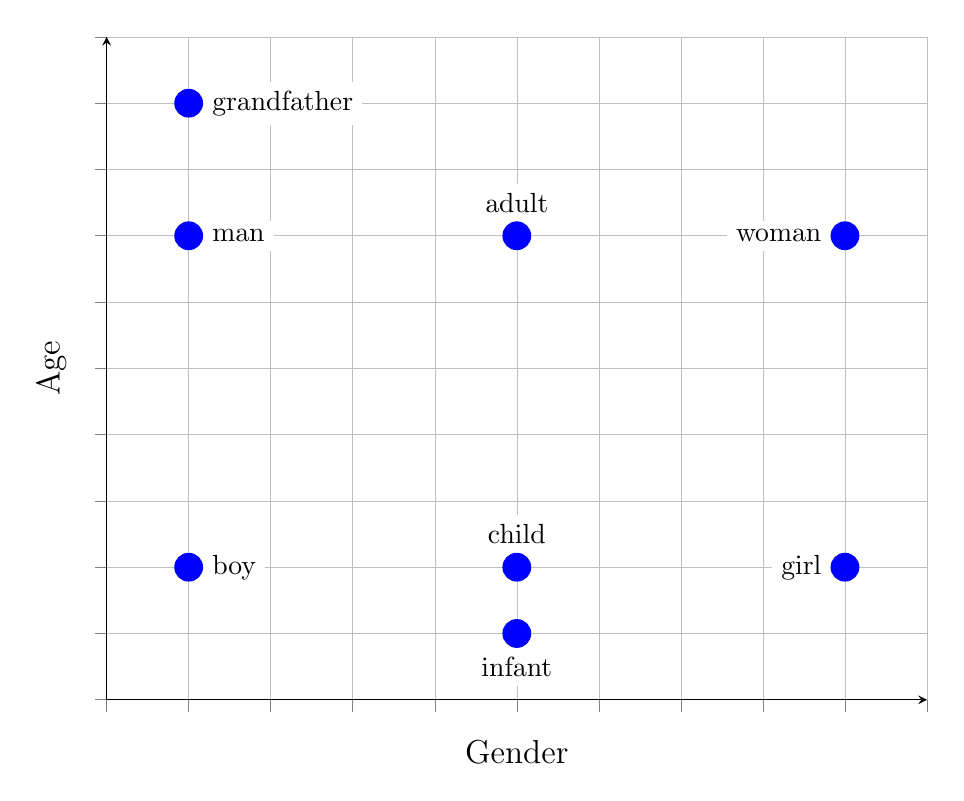
\begin{tikzpicture}
  \begin{axis}[
      width=12cm, height=10cm,
      xlabel={Gender}, ylabel={Age},
      xmin=0, xmax=10, ymin=0, ymax=10,
      xtick={0,1,...,10}, ytick={0,1,...,10},
      xticklabel={\empty}, yticklabel={\empty},
      grid=both,
      grid style={line width=.1pt, draw=gray!30},
      major grid style={line width=.2pt,draw=gray!50},
      axis lines=left,
      tick align=outside,
      enlargelimits=false,
      label style={font=\large},
      title style={font=\LARGE, yshift=1em},
      every tick label/.append style={font=\small},
    ]

    % Plot the points
    \addplot[
      only marks,
      mark=*,
      mark size=5pt,
      blue,
    ] coordinates {
        (1,9)   % grandfather
        (1,7)   % man
        (1,2)   % boy
        (5,7)   % adult
        (5,2)   % child
        (5,1)   % infant
        (9,7)   % woman
        (9,2)   % girl
      };

    % Add labels
    \node[fill=white, anchor=west, xshift=5pt, font=\normalsize] at (axis cs:1,9)  {grandfather};
    \node[fill=white, anchor=west, xshift=5pt, font=\normalsize] at (axis cs:1,7)  {man};
    \node[fill=white, anchor=west, xshift=5pt, font=\normalsize] at (axis cs:1,2)  {boy};
    \node[fill=white, anchor=south, yshift=5pt, font=\normalsize] at (axis cs:5,7)  {adult};
    \node[fill=white, anchor=south, yshift=5pt, font=\normalsize] at (axis cs:5,2)  {child};
    \node[fill=white, anchor=north, yshift=-5pt, font=\normalsize] at (axis cs:5,1)  {infant};
    \node[fill=white, anchor=east, xshift=-5pt, font=\normalsize] at (axis cs:9,7)  {woman};
    \node[fill=white, anchor=east, xshift=-5pt, font=\normalsize] at (axis cs:9,2)  {girl};
  \end{axis}
\end{tikzpicture}
  \end{center}
  \caption{TODO:}
  \label{fig:embeddings} % TODO: reference
\end{figure}

Early models for word representation focused on learning fixed vectors for each word, resulting in what are known as static word embeddings. These embeddings assign the same vector to a word regardless of the context in which it appears. Well-known examples of such approaches include Word2Vec (\cite{mikolovEfficientEstimationWord2013}) and GloVe (\cite{penningtonGloveGlobalVectors2014}), both of which capture semantic similarities based on word co-occurrence statistics in large text corpora.

Although static word embeddings are computationally efficient and useful in many scenarios, they are unable to account for variations in meaning across different contexts. This limitation has led to the development of contextual word embeddings, which are context-dependent. One early example is ELMo (\cite{petersDeepContextualizedWord2018}), which uses bidirectional \ac{lstm} networks to generate embeddings sensitive to surrounding words in a sentence.

More recent approaches use transformer-based architectures. Models such as BERT (\cite{devlin-etal-2019-bert}) generate deep contextual embeddings using self-attention mechanisms to model relationships between words within a given context. Contextual information is crucial because it enables models to disambiguate polysemous words. For example, the word \enquote{bank} can refer to a financial institution or the side of a river, and only contextual clues can determine the intended meaning.

These contextual embeddings have substantially improved performance across a wide variety of \ac{nlp} tasks, including question answering, named entity recognition, and machine translation. As a result, they have become essential components of modern \ac{nlp} pipelines.

\section{Stylistic Investigations}
\label{sec:background:styleInvestigations}
% TODO: write a little more about the proxy tasks; what are they, what are examples, why are they necessary
% TODO: example for learned style embedding method with citation
The objective of Stylistic Investigations is to identify an author's unique writing style independent of the content being expressed. Modern neural approaches often accomplish this by learning dense vector representations, or style embeddings, through proxy tasks. These tasks include style transfer, authorship attribution or verification, and group membership detection. Proxy tasks enable models to learn stylistic features without explicit style annotations. This is important because annotating large amounts of data is very difficult and time-consuming.

However, one drawback of learned style embeddings is that it is difficult to ensure that the representations are truly independent of the content, as noted by \citet{wegmannSameAuthorJust2022}. This complicates their application in new domains where the content may differ. Additionally, such embeddings tend to be uninterpretable, reducing their transparency and limiting their usefulness in downstream tasks.

Some approaches aim to produce interpretable embeddings to address these issues. Notable examples include the work by \citet{patelLearningInterpretableStyle2023}, who propose a method for learning attribute-based representations, and \citet{alshomaryLatentSpaceInterpretation2024}, who focus on interpreting latent embeddings. This thesis builds on and extends this line of research by proposing a new method for learning interpretable style embeddings that incorporate knowledge-related dimensions.

Other, more classical methods for stylistic analysis take a different approach. They work by manually selecting interpretable features such as the frequency of function words, syntactic structures, or punctuation counts. These features are extracted using comprehensible algorithms and can be used to construct explainable classifiers, although they may lack the nuance and representational capacity of neural embeddings.
\citet{okulskaStyloMetrixOpensourceMultilingual2023} presented Stylometrix as an example of recent work in this area. It generates interpretable style vectors based on a curated set of features. Another example is StyloAI, which was developed \citet{oparaStyloAIDistinguishingAIgenerated2024a} and extracts 31 stylometric features to identify AI-generated texts using a Random Forest classifier.

The main advantages of feature-based approaches are the relevance and quality of the extracted features. However, these methods have several drawbacks. First, they require manual feature selection, which limits the range of stylistic attributes that can be captured. Additionally, these methods cannot incorporate more abstract attributes requiring a deeper understanding of the text, such as the knowledge-related features employed in this thesis.

\section{Large Language Models}
\label{sec:background:llm}

\Acfp{llm} are large-scale neural networks with billions of parameters. These models are pre-trained on massive text corpora and can perform tasks that require advanced language understanding and generation (\cite{minaeeLargeLanguageModels2025}).
\acp{llm} have brought significant advancements to the field of \acl{nlp}, achieving state-of-the-art performance in a broad range of applications. These include text generation, translation, and question answering, among many others.

The transformer architecture, introduced by \citet{NIPS2017_3f5ee243} in the seminal paper \enquote{Attention Is All You Need}, is the foundation of most modern \acp{llm}. Unlike earlier models, which relied on recurrence or convolution, the transformer architecture uses self-attention mechanisms to weigh the relevance of each word in the input sequence relative to the others. This design supports parallel processing, thereby improving training efficiency and scalability.

As shown in Figure~\ref{fig:transformerArchitecture}, the transformer follows an encoder-decoder architecture. The encoder processes the input sequence and produces a continuous representation. Then, the decoder generates the output sequence based on the encoder's output and previous outputs. There are encoder-only models, such as embedding models, that produce a representation of the input text. There are also decoder-only models that predict subsequent tokens based on previous outputs or a prompt.

This thesis will employ encoder-only models to create interpretable attribute embeddings. Decoder-only \acp{llm} will be used for the task of text generation.

\begin{figure}[ht]
  \begin{center}
    \input{figures/tikz/transformer-architecture.tex}
  \end{center}
  \caption{TODO:} % TODO: mention source (attention is all you need); explain layers
  % source: https://www.cs.cmu.edu/~dst/WordEmbeddingDemo/tutorial.html
  \label{fig:transformerArchitecture}
\end{figure}

\section{Steering of Large Language Models}
\label{sec:background:llm:steering}

Although \acp{llm} are highly effective at generating coherent and fluent text, it is often desirable to guide the generated text to follow specific constraints or stylistic forms. It is also essential to prevent models from generating toxic or inappropriate content. Several steering methods have been developed to address these challenges.

One widely used method is \textbf{prompt engineering}, which involves steering the model by modifying the input prompt provided during inference. The key advantage of this approach is that it does not require any model training (\cite{schulhoffPromptReportSystematic2024}).

There are several variations of prompt engineering. One important type involves changing the system prompt, which is particularly relevant in chat-based \acp{llm}. A system prompt defines how a model behaves and what tone it uses throughout a conversation. Although it is hidden from the user, the system prompt can influence the model to adopt a specific persona, adhere to formatting rules, or follow safety guidelines. For instance, the system prompt can instruct the model to act as a helpful tutor or avoid discussing certain topics. This steering technique will be evaluated in this thesis.

Another variant of prompt engineering is few-shot prompting. With this approach, the prompt contains instructions for the task and a few examples of correct task completions. These examples allow the model to generalize to similar tasks by recognizing patterns.

% chain-of-thought prompting by Wei et al., 2022 % TODO: include this?

\textbf{Fine-tuning} is a more resource-intensive method of steering that involves updating the parameters of the model using task-specific data. Although fine-tuning can yield strong performance, it is often too expensive for \acp{llm} due to their size. Furthermore, using a different fine-tuned model for each task can be inefficient and impractical.

To mitigate these issues, parameter-efficient fine-tuning methods have been developed. These methods freeze the pre-trained model weights and only train a small number of additional parameters. One such method is prefix tuning (\cite{liPrefixtuningOptimizingContinuous2021}), where a learned vector (prefix) is prepended to the model input. This method achieves competitive performance while training only \SI{0.1}{\percent} of the model's parameters. Another example is LoRA (\cite{huLoRALowrankAdaptation2021}), which introduces trainable low-rank matrices into the model while keeping the original weights fixed. LoRA reduces the number of trainable parameters by a factor of \num{10000} without compromising performance.

% \textbf{Reinforcement Learning from Human Feedback (RLHF)} % TODO: include this?

A recent alternative to these methods is \textbf{activation steering}, which directly alters the hidden states of an \acs{llm} during inference to guide its output. These hidden states are generally accessed at the end of each transformer layer. Modern \acp{llm} typically consist of between \num{20} and \num{100} such layers, with deeper layers typically encoding more abstract and sophisticated concepts (\cite{bogdanEmergentEffectsScaling2025}).

Activation steering involves identifying and extracting the hidden states that correspond to specific concepts in a single forward pass. These extracted vectors, known as steering vectors, are added to the internal states of the model during inference to guide the generation process in the desired direction (\cite{konenStyleVectorsSteering2024,turnerActivationAdditionSteering2024,subramaniExtractingLatentSteering2022}).

\clearpage

\chapter{Datasets}%
\label{sec:datasets}

\section{Stack Exchange Dataset}%
\label{sec:datasets:stackex}

\begin{itemize}
  \item main dataset used in this thesis
  \item taken from Stack Exchange\footnote{TODO}, an online forum
  \item taken from sub forums that are group specific
\end{itemize}

\section{AskX Dataset}%
\label{sec:datasets:askx}
% We derive this corpus from Reddit, an online discussion forum in which users publicly post messages to which other users post responses. Reddit is structured into subreddits, each of which focuses on a specific topic, has subreddit-specific posting rules, and subredditspecific moderators that enforce these rules. We consider a specific kind of subreddit that follows the "AskX" schema. Examples of such subreddits are "AskAGerman" and "AskAnAmerican". As per the rules of these subreddits, anyone can ask a question, but only members of the specific demographic should answer these questions. So, in "AskAGerman", all answers should be written by German nationals. We identified 91 subreddits that follow the AskX schema. From these, we manually selected 13 AskX subreddits from which to derive a corpus (see Table 1).


\section{Steering Dataset}%
\label{sec:datasets:steering}
\begin{itemize}
  \item questions taken from \citet{petroni-etal-2021-kilt,rooeinKnowYourAudience2023}
\end{itemize}

\clearpage

% !TeX root = ..\..\thesis.tex
\chapter{Approach}
\label{sec:approach}

This thesis proposes a method to create an interpretable attribute vector which can be used for group membership detection. Furthermore, different methods to steer the output of \acp{llm} are presented which will be used to create group specific explanations for various topics. The interpretable attribute vector will be used for the steering process as well as its evaluation.

The dimensions of the attribute vector are values between \num{0} and \num{1} where each dimension corresponds to an attribute sentence with a real world meaning.

Previous work by \citet{patelLearningInterpretableStyle2023,alshomaryLatentSpaceInterpretation2024} focus on stylistic attributes for authorship attribution tasks. In this thesis, I will extend the style vector by knowledge attributes, which focus on the experience and background knowledge of the author. While these attributes are not as important for authorship attribution or group membership detection tasks, they will be helpful to steer explanations towards the appropriate knowledge level for specific groups of people. The style and knowledge attributes together form the attribute vector.
% TODO: explain why the knowledge attributes are important

\section{Attribute Sentence Generation}
\label{sec:approach:attributeSentenceGeneration}

The attribute sentences that form the dimensions of the interpretable attribute vector are generated by prompting a \acf{llm} in a two-step procedure.

For step one, the \ac{llm} is presented with a zero-shot prompt to produce a description of the text. This step is repeated \num{\numPrompts} times, each time with a different prompt that focuses on a specific aspect of the text. \num{\numOpenPrompts} prompts (see Appendix~\ref{sec:appendix:openPrompts}) are relatively open and only give a loose direction on which style should be described by the model. \num{\numTargetPrompts} prompts (see Appendix~\ref{sec:appendix:targetPrompts}) are targeted towards an explicit stylistic feature. These prompts follow the work of \citet{patelLearningInterpretableStyle2023,tausczikPsychologicalMeaningWords2010} to get the model to focus on a broad variety of styles that are important for the study of language.
In contrast to the method presented by \cite{patelLearningInterpretableStyle2023}, there are \num{\numKnowledgePrompts} prompts (see Appendix~\ref{sec:appendix:knowledgePrompts}) which focus on the knowledge and experience of the author in addition to the style prompts.
% While the author's background knowledge is not as important for group membership detection as the style of the text, it is helpful information for the steering task covered in later sections. % already written in introduction of approach

After generating the descriptions, the \ac{llm} is prompted a second time to rewrite them as a list of sentences. The model is instructed to write each sentence in a consistent form like \enquote{The author is \ldots} or \enquote{The author uses \ldots}. This process is shown in Figure~\ref{fig:attributeSentenceGeneration}.

\begin{figure}[ht]
  \newlength{\mytw}
\settowidth{\mytw}{A few lines of text in a block}
\begin{center}
  \begin{tikzpicture}
    [> = latex', auto,
      block/.style ={
          rectangle,
          draw=black,
          thick,
          % align=flush center,
          rounded corners,
          % minimum height=4em
        },
    ]
    \node[block, text width=0.7\linewidth] (answer) {\textbf{Input Text:}\\If the judge believes the award is too high or too low, the judge can use additur or remittitur to reduce the damages. These are essentially offers to both parties to agree to the change in damages. If both parties do not agree, the court can order a new trial.};

    \node[block, minimum height=3cm, text width=0.4\linewidth, below left=of answer.south] (prompt1) {\textbf{Prompt 1 (Grammar Style):}\\Write a long paragraph describing the unique grammar style of the following passage without referring to specifics about the topic.};
    \node[align=flush center, minimum height=3cm, text width=0.2\linewidth, below=1cm of answer.south] (prompt2) {\ldots};
    \node[block, minimum height=3cm, text width=0.4\linewidth, below right=of answer.south] (prompt3) {\textbf{Prompt 92 (Background Knowledge):}\\Write a description of the background knowledge the author has based on the following passage.};

    \draw[->] (answer.south) -- (prompt1.north);
    \draw[->] (answer.south) -- (prompt2.north);
    \draw[->] (answer.south) -- (prompt3.north);

    \node[block, align=flush center, minimum height=1cm, text width=0.4\linewidth, below=1cm of prompt1] (description1) {Style Description};
    \node[align=flush center, minimum height=1cm, text width=0.2\linewidth, below=1cm of prompt2] (description2) {\ldots};
    \node[block, align=flush center, minimum height=1cm, text width=0.4\linewidth, below=1cm of prompt3] (description3) {Style Description};

    \draw[->] (prompt1.south) -- (description1.north);
    \draw[->] (prompt2.south) -- (description2.north);
    \draw[->] (prompt3.south) -- (description3.north);

    \node[block, text width=0.95\linewidth, below=1cm of description2] (sentence_prompt) {\textbf{Prompt:}\\Rewrite this description as a long list of short sentences describing the author's writing style  where each sentence is in the format of \enquote{The author is X.} or \enquote{The author uses X.}.};

    \draw[->] (description1.south) -- ++(0,-1cm);
    \draw[->] (description2.south) -- ++(0,-1cm);
    \draw[->] (description3.south) -- ++(0,-1cm);

    \node[block, text width=0.95\linewidth, below=1cm of sentence_prompt] (attributes) {\textbf{Style Attributes:}\\
      % The author uses the passive voice. \\
      % The author uses active voice. \\
      % The author uses sentence fragments. \\
      % The author uses run-on sentences. \\
      % The author uses words related to visual perception. \\
      % The author uses words expressing wellness. \\
      % The author uses a neutral tone. \\
      The author uses words related to risk. \\
      % The author uses words related to allure. \\
      % The author uses words indicating poverty. \\
      The author uses words expressing needs. \\
      % The author uses numbers. \\
      The author explains legal concepts. \\
      % The author uses words indicating men. \\
      The author uses the word judge. \\
      \ldots
    };

    \draw[->] (sentence_prompt.south) -- +(0,-1cm);
    \draw[->] let \p1 = (sentence_prompt.south), \p2 = (description1) in (\x2,\y1) -- +(0,-1cm);
    \draw[->] let \p1 = (sentence_prompt.south), \p2 = (description3) in (\x2,\y1) -- +(0,-1cm);
  \end{tikzpicture}
\end{center}

  % TODO: better caption
  \caption{The process to generate attribute sentences.}
  \label{fig:attributeSentenceGeneration}
\end{figure}

In addition to the requirement towards the shape of the sentences, the model is instructed to avoid negations and examples since these both lead to increasing problems with the clustering process that is described in Section~\ref{sec:approach:clustering}.
Sentences that include examples are potentially problematic because it increases the likelihood of sentences which have the same content while being of significantly different shape; an example for this problem would be the sentences \enquote{The author uses filler words} and \enquote{The author uses filler words such as 'and', 'or' and 'furthermore'}. While this problem will be reduced by clustering similar sentences, the procedure is not perfect and will be more robust if the model avoids sentences with examples.

Negations, on the other hand, lead to the problem where the shape of the sentences will be too close while the content is very different. There is a high chance that the sentences \enquote{The author does use long sentences} and \enquote{The author does not use long sentences} will be clustered together because so much of them is the same, even though they state the opposite of each other.
Additionally, the dimensions of the final attribute vector should not include any negated attributes since the expression \enquote{The author uses short sentences} is much clearer than \enquote{The author does not use long sentences}.

Since the model might produce sentences with negations or examples despite the prompt, each of the generated sentences is also automatically checked before further processing, following the work of \citet{patelLearningInterpretableStyle2023}.

Per description, each distinct attribute sentence is recorded only once, even if the model generates it multiple times. This is done in case the model generates a bad answer where one sentence is repeated many times.


\section{Clustering}
\label{sec:approach:clustering}
A strength of the method to create attribute sentences described in Section~\ref{sec:approach:attributeSentenceGeneration} is the lack of constraints which results in a large variety of generated sentences. However, this leads to the problem that sentences with the same content can have many different shapes. An example for this would be the sentences \enquote{The author uses short and concise sentences.} and \enquote{The author uses concise and short sentences.}, which have the same meaning while being considered as two completely different sentences by the procedure up to this point.

Because of that, it is more difficult to compare different input texts and to find texts that fit a similar feature attribute.
% Additionally, the selection of the dimension of the attribute vector described in Section~\ref{sec:approach:selection} could become more difficult as the number of times that an attribute has been used is obscured. % maybe other wording, but probably don't reference future sections
To solve this problem, my approach includes clustering the sentences by the cosine similarity of their embeddings, which are produced by a sentence embedding model.

The clustering algorithm first computes a radius neighbor graph of all sentences. The sentences that have a sufficiently high cosine similarity are considered to be in the same cluster. Subsequently, the clusters are sorted by size and inspected from largest to smallest. If a sentence is included in one cluster, it is removed from all smaller ones. It is important to note that there is no minimum size for a cluster; if a sentence has no neighbors or every one of them is already part of a larger cluster, then the cluster size is one.

The sentence that is closest to the center of each cluster represents it. When the cluster is used, this sentence and its embedding are actually used.

This process is carried out separately for sentences that have been produced by style prompts and those produced by knowledge prompts (see Section~\ref{sec:approach:attributeSentenceGeneration}). Otherwise, it could happen that a cluster includes lots of knowledge sentences, but the center sentence is a style sentence, which could cause some problems in the later stages of the approach. % TODO: mention steering?
The resulting clusters are referred to as style clusters and knowledge clusters.


\section{Training and Testing \acs{sfam}}
\label{sec:approach:sfam}

The goal of the method presented in this thesis is to create interpretable attribute vectors with values between \num{0} and \num{1} that correspond to real-world values. To create these values, a model will be trained which follows the \acf{sfam} that was presented by \citet{patelLearningInterpretableStyle2023}. It takes an attribute sentence and a text and outputs an agreement score that corresponds to how well the attribute sentence fits the text.

\ac{sfam} is trained on the synthetic dataset, which was created in earlier steps as described in Section~\ref{sec:approach:attributeSentenceGeneration}. The training data includes the unclustered knowledge and style sentences and the input texts that were described by them. There is however some preprocessing necessary, because just because an attribute sentence was not used to describe a text does not mean the text does not match the sentence. It could be that the text was described by a similar sentence or that the \ac{llm} just skipped a topic when describing one text.

The attribute sentences that are used for training are selected in a process similar to the one described in Section~\ref{sec:approach:selection:finalSelection}.
First, the similarity between all attribute sentences and all attribute vector dimensions is computed. Then, for each sentence and each text, the average similarity to the dimensions that were used to describe the text is computed. The texts are then sorted by their similarity to the attribute sentence. If the sentence has been used to describe one of the \SI{1}{\percent} most similar texts, this text will be used as a positive training sample, and the most dissimilar text where the sentence was not used to describe it is used as a negative training sample. Otherwise, the sentence will not be used for training.

The resulting dataset is balanced regarding positive and negative samples and has a high probability of only including sentences that fit the texts. % TODO: write better
The same process is used to create the validation and test datasets using different answers. % TODO: write here that the attribute sentences are largely distinct or later in experiments?

% \begin{itemize}
%   \item \ac{sfam} is a model that takes a style sentence and a text as input and produces an agreement score
%   \item training data
%         \begin{itemize}
%           % \item the \numStyleSentences{} style sentences are used for training % do not use numbers for approach
%           \item there are distinct sets of input texts for training, validation and test datasets
%           \item these lead to mostly different sentences (also the differences may be small)
%           \item of all sentences, the best are selected
%                 \begin{itemize}
%                   \item compute similarity to all style vector attributes (which are clusters)
%                   \item for each sentence, compute the most similar and most dissimilar input text according to the average similarity to all style attributes that have been used to describe that text (like the final selection of style vector attributes, see Section~\ref{sec:approach:selection}) % TODO: is there a more specific reference to a subsection?
%                   \item if one of the ten most similar input texts was actually described by the style sentence, it is chosen as a positive training sample and the least similar input text that was not described by the sentence as a negative sample
%                   \item otherwise, the sentence is not used for training
%                   \item the same is done for validation and test
%                 \end{itemize}
%         \end{itemize}
%   \item \ac{sfam} is a finetuned DeBERTaV3 model
%         \begin{itemize}
%           \item two fully connected layers with a ReLu in between % TODO: look up
%           \item finally a sigmoid activation function to produce values between 0 and 1
%         \end{itemize}
%   \item optional hyperparameter optimization (with optuna -> citation?) to discover optimal learning rate and weight decay
%   \item early stopping callback with patience of three
%   \item validation metric of accuracy
%   \item testing metric accuracy and f1
% \end{itemize}


\section{Training and Testing \acs{lisa}}
\label{sec:approach:lisa}
While \ac{sfam} produces the Attribute Vector with exactly the values that are required, it needs one forward pass per dimension of the vector. Even with an optimized model, this takes too long a time for most applications. The solution is to train an additional model, the \acf{lisa} model proposed by \citet{patelLearningInterpretableStyle2023}, which gets a text as input and produces the full attribute vector in one forward pass.

The training, validation, and test data are created by using \ac{sfam} to create the Attribute Vectors of the corresponding texts and training \ac{lisa} as a regression model.

% \begin{itemize}
%   \item to get values for a style vector, the \num{\styleVectorSize} forward passes by \ac{sfam} would take too long for most practical applications
%   \item train an additional model that creates the whole vector in one forward pass
%   \item \ac{lisa} like \ac{sfam} is a finetuned DeBERTaV3 model
%         \begin{itemize}
%           \item two fully connected layers with a ReLu in between % TODO: look up
%           \item finally a sigmoid activation function to produce values between 0 and 1
%         \end{itemize}
% \end{itemize}

\section{Embedding Model}
\label{sec:approach:embedding}
The \ac{lisa} model produces an attribute vector where each dimension corresponds to one attribute sentence. The problem with this vector is that two vectors can not be easily compared to each other because the dimensions are not normalized and have different importance for the meaning of the vector.

Because of that, an embedding head for the \ac{lisa} model is trained that produces attribute embeddings. While the dimensions of the embedding are not directly interpretable, they are derived directly from the interpretable attribute vectors and therefore do not lose much interpretability.

\section{Steering Text Generation}
The aim of this thesis is to combine the group membership task with the steering of \acp{llm} towards group-specific explanations. Multiple different methods will be presented and compared to each other. The method is split into two groups: changing the system prompt to steer the model and manipulating the output of the activation functions after selected layers.

\subsection{Prompt Steering}
\label{sec:approach:steering:prompt}
I will be looking at three different methods of changing the system prompt to adapt the way the \ac{llm} answers questions by the user to match a specific group.

The first and simplest way to change the system prompt is to instruct the model to write an explanation for a specified group. In this case, the system prompt includes the following sentence:
\begin{quote}
  You are an author who writes a helpful explanation for a group of <group>.
\end{quote}

While this method can not be influenced regarding the direction or strength of the steering effect, it is very easy to implement and will serve as a baseline to compare the other steering methods against.

For the second prompt steering approach, the data that is used to extract the features of the attribute vector as described in Section~\ref{sec:approach:attributeSentenceGeneration} will be used to determine the most important attributes that differentiate each group from all the others. The most important style and knowledge attribute will then be a part of the system prompt.

For the attributes to be able to be effectively used in the system prompt, they can not be of the form \enquote{The author is \ldots}. Instead, the attributes are automatically rewritten to address the model directly, as this role-playing is a strength of modern \aclp{llm}. % TODO: citation
Thus, the attribute sentences will have the form \enquote{You are \ldots}.

The final prompt steering methods will combine the two previous methods and include both the group name and the most important attribute sentences in the system prompt.

\section{Activation Steering}

While the prompt steering methods are easy to implement, they have the disadvantage that they do not allow for fine-grained steering. Even when the most important attributes are included in the system prompt, there is no way to tell the model how strongly each attribute should influence the generated text. To solve this problem, this thesis proposes a method to steer the \ac{llm} by manipulating its activation space during inference following the work of \citet{turnerActivationAdditionSteering2024,rimsky-etal-2024-steering}.

The steering vectors are created without any training process, which reduces the required time significantly. For each dimension of the interpretable attribute vector, a separate steering vector is extracted.

\begin{figure}[ht]
  \begin{tikzpicture}[
    >=Stealth,
    attr/.style={
        matrix of nodes,
        nodes={anchor=base west, font=\footnotesize},
        row sep=3pt,
        inner sep=6pt,
        nodes in empty cells,
        draw, rectangle,
        anchor=north west
      },
    % steering‐vector boxes:
    sv/.style={draw, rectangle, minimum width=3cm, align=center},
    % generic box:
    box/.style={draw, rectangle}
  ]

  % 2) Attribute‐vector matrix (flush)
  \matrix[attr] (attrvec)
  at (0,0)
  {
    \num{0.653}         \\
    \num{0.934}         \\
    \num{0.845}         \\
    \num{0.103}         \\
    $\dots$\vphantom{0} \\
  };
  \node[above=2pt of attrvec.north] {\small\bfseries Attribute Vector};

  \node[anchor=west] (feature1) at (attrvec.east |- attrvec-1-1.center) {The author uses a positive tone.};
  \node[anchor=west] (feature2) at (attrvec.east |- attrvec-2-1.center) {The author uses long sentences.};
  \node[anchor=west] (feature3) at (attrvec.east |- attrvec-3-1.center) {The author uses technical terms.};
  \node[anchor=west] (feature4) at (attrvec.east |- attrvec-4-1.center) {The author uses code snippets.};
  \node[anchor=west] (feature5) at (attrvec.east |- attrvec-5-1.center) {\dots};

  % 3) Steering‐vector x‐position
  \coordinate (steerBase) at ($(feature1.east)+(5cm,0)$);

  % 4) Midpoint for floating “Extraction” box
  \coordinate (midX)      at ($(feature1.east)!.5!(steerBase.west)$);

  % 6) Steering vectors aligned row‐wise
  \foreach \i in {1,...,4} {
      \node[sv] (sv\i) at (steerBase |- feature\i) {Steering Vector};
    }
  \node[sv] (sv5) at (steerBase |- feature5) {\dots\vphantom{Steering Vector}};

  % 7) Softmax matrix
  \matrix (softmax) [
    attr,
    below right=2cm and 2cm of feature4.south east
  ] {
    \num{0.098}       \\
    \num{0.201}       \\
    \num{0.121}       \\
    \num{0.001}       \\
    \dots\vphantom{0} \\
  };

  %––––––––––––––––––––––––––––––––––––––––––––––––––––––––––––––
  % A) Extraction arrows: from attrvec numbers → each sv
  \foreach \i in {1,...,5} {
      \draw[->] (feature3.east |- feature\i) -- (sv\i.west);
    }

  % 5) Floating “Extraction” box (dashed)
  \node[box, dashed, fill=white, minimum height=3.5cm, anchor=north, align=center]
  at ($(midX)+(-0.7cm,0.2cm)$)
  (extraction) {Extraction}; % {Activation\\Vector\\Extraction}

  % B) Features → Softmax
  % \draw[->] (attrvec.south) |-  (softmax.north);
  \draw[<-] let
  \p1 = (softmax.north),
  \p2 = (attrvec)
  in (softmax.north) -- ++(0, 0.5cm) node at ({(\x1 + \x2)/2}, {\y1 + 0.8cm}) {Softmax} -| (attrvec.south);

  % C) SVs → Softmax entries
  \foreach \i in {1,...,5} {
      \draw[->] let \p1 = (softmax.east), \p2 = (softmax-\i-1.east) in (sv\i.east) -- ++({0.25cm * \i}, 0) |- (\x1, \y2);
    }

  % 8) Sum + group Steering Vector
  \node[draw,circle,left=2cm of softmax-3-1] (sum) {+};
  \node[sv,left=of sum] (group) {Group Steering Vector};

  % D) Softmax → Sum → Group
  \foreach \i in {1,...,5} {
      \draw[] (softmax.west |- softmax-\i-1.west) -- (sum.east);
    }
  \draw[->] (sum.west) -- (group.east);

\end{tikzpicture}

  \label{fig:activationSteering}
  \caption{Todo}
\end{figure}

\subsubsection{Extracting Steering Vectors}
The attribute that should be steered towards will be a part of the system prompt similar to the prompt attribute steering described in Section~\ref{sec:approach:steering:prompt}. Following that, the model predicts the next token in one forward pass. From that inference, the vectors after the activation functions of each layer are extracted and saved. The predicted token is not important during this process. % TODO: extract from activation functions or from residual streams?

To get the steering vector of a group, all attribute steering vectors need to be combined. For that, a softmax of the median attribute vector for a group is created. Afterward, each attribute steering vector is multiplied with the corresponding value of the softmax. Finally, all weighted steering vectors are added together.

Alternatively, instead of including all dimensions of the attribute vector, only the most important attributes can be used to create the group steering vector.

\subsubsection{Text Generation Steering}
\label{sec:approach:steering:activation}
To steer the text generation of a \acl{llm}, the computed steering vector is added to a layer of the model during the forward pass. The layer the vector is inserted into must be the same as the vectors that were combined to form the steering vector where taken from. The steering vector can be scaled with a factor \(\lambda\) to further control the strength of the steering effect.
Because the steering vector is extracted during the first forward pass, it is also inserted exclusively during the first forward pass (\cite{rimsky-etal-2024-steering}).
% \begin{itemize}
%   \item strength of the method is that no training is needed
%   \item the activation vectors will be extracted at each layer
%   \item for each attribute vector dimension, an activation vector is extracted
%   \item to create the steering vector for the layer x
%         \begin{enumerate}
%           \item take the attribute vector (for example for a group)
%           \item take a softmax
%           \item multiply the activation vector of each attribute sentence with the corresponding softmax value
%           \item add the weighted activation vectors together
%           \item multiply them with a factor \(\lambda\)
%         \end{enumerate}
%   \item the steering vector is added to the activation vector at layer x during the forward pass of a steered text generation
% \end{itemize}

\clearpage
\section{For Leandra}

The table from the presentation:

\begin{tabular}{lSS}
  \toprule
  {Group}              & {Euclidean\ Distance}                              & {Cosine\ Similarity}                               \\
  \midrule
  Biologists           & 1.5506118535995483                                 & 0.33786728978157043                                \\
  Data Scientists      & 2.1414427757263184                                 & 0.49583321809768677                                \\
  Electrical Engineers & 1.334580421447754                                  & 0.03393082693219185                                \\
  Game Developers      & 1.4480421543121338                                 & 0.044030994176864624                               \\
  Lawyers              & 3.108609199523926                                  & \cellcolor[gray]{0.8} \bfseries 0.8223204016685486 \\
  Philosophers         & 2.6420016288757324                                 & 0.7476155757904053                                 \\
  Politicians          & \cellcolor[gray]{0.8} \bfseries 3.1334586143493652 & 0.7666002511978149                                 \\
  Software Engineers   & 1.611264705657959                                  & 0.2527718245983124                                 \\
  \bottomrule
\end{tabular}

The table with the new metrics:

\resizebox{\linewidth}{!}{
  \begin{tabular}{lSSSS}
    \toprule
    {Group}              & {Steering Effect}                                  & {Direction Correctness}                            & {Possible Steering Effect}                        & {Distance Difference}                              \\
    \midrule
    Astronomers          & 1.7484214305877686                                 & 0.5161562561988831                                 & 7.244743824005127                                 & 5.496322154998779                                  \\
    Pilots               & 1.7315958738327026                                 & 0.5180053114891052                                 & 8.215267181396484                                 & 6.483670711517334                                  \\
    Biologists           & 1.5506118535995483                                 & 0.38158202171325684                                & 5.649219989776611                                 & 4.098607063293457                                  \\
    Chemists             & 1.5814242362976074                                 & 0.3781886696815491                                 & 8.697698593139648                                 & 7.116274833679199                                  \\
    Cryptographers       & 2.203723192214966                                  & 0.4798935353755951                                 & 11.444587707519531                                & 9.240863800048828                                  \\
    Computer Scientists  & 1.6375644207000732                                 & 0.3859226703643799                                 & 7.956028938293457                                 & 6.3184638023376465                                 \\
    Data Scientists      & 2.1414427757263184                                 & 0.6237024068832397                                 & 10.039475440979004                                & 7.898032188415527                                  \\
    Electrical Engineers & 1.334580421447754                                  & -0.038641635328531265                              & 7.1854705810546875                                & 5.850890636444092                                  \\
    Game Developers      & 1.4480421543121338                                 & 0.1651124805212021                                 & 7.710322856903076                                 & 6.262280464172363                                  \\
    Historians           & 1.5222752094268799                                 & 0.509942352771759                                  & 12.36848258972168                                 & \cellcolor[gray]{0.8} \bfseries 10.846207618713379 \\
    Lawyers              & 3.108609199523926                                  & 0.7886425852775574                                 & \cellcolor[gray]{0.8} \bfseries 13.44083023071289 & 10.332222938537598                                 \\
    Mechanical Engineers & 1.676805853843689                                  & 0.5361155867576599                                 & 11.346585273742676                                & 9.669781684875488                                  \\
    Philosophers         & 2.6420016288757324                                 & 0.8240012526512146                                 & 10.290709495544434                                & 7.648707866668701                                  \\
    Physicists           & 1.5092840194702148                                 & 0.4641623795032501                                 & 6.5638251304626465                                & 5.054540634155273                                  \\
    Politicians          & \cellcolor[gray]{0.8} \bfseries 3.1334586143493652 & \cellcolor[gray]{0.8} \bfseries 0.8509434461593628 & 12.980879783630371                                & 9.847421646118164                                  \\
    Software Engineers   & 1.611264705657959                                  & 0.34105777740478516                                & 8.732571601867676                                 & 7.12130880355835                                   \\
    \bottomrule
  \end{tabular}
}

As expected, the direction is sometimes better and sometimes worse, but roughly the same.
\clearpage

\chapter{Experiments}
\label{sec:experiments}

\section{Environment and Hardware}
\label{sec:experiments:environmentHardware}
The experiments were conducted on a SLURM cluster using nodes with \num{32} CPU cores, \SI{128}{\giga\byte} RAM and an Nvidia A-100 GPU with \SI{40}{\giga\byte} VRAM. The implementation is written in python 3.10.13. The data is stored in a SQLite database, the database schema can be found in Appendix~\ref{sec:appendix:databaseSchema}.

\section{Experimental Setup}
\label{sec:experiments:setup}

% TODO: introduction

\subsection{Attribute Sentence Generation}
\label{sec:experiments:setup:sentenceGeneration}
The synthetic dataset that consists of attribute sentences which describe a set of input texts is constructed by prompting an \acs{llm} in a two-step procedure. For this thesis, the open source model Llama 3.2 Instruct\footnote{\url{https://huggingface.co/meta-llama/Llama-3.2-3B-Instruct}}~(\cite{dubeyLlama3Herd2024}) with \num{3} billion parameters has been used. This model has state-of-the-art performance and is freely available, which provides the possibility to run the model directly on the server cluster. Additionally, it improves the reproducibility of the experiments because it is easier to use the exact same model later.
To improve the performance of the sentence generation, the library vLLM\footnote{\url{https://github.com/vllm-project/vllm}} was used to run the model.

The basis for the generation of the attribute sentences are \num{\numAnswersStyleVector} answers from the stack exchange dataset described in Section %~\ref{}. TODO:
For each of the answers, the model is prompted \num{\numPrompts} times to create descriptions of the text with the method presented in Section~\ref{sec:approach:attributeSentenceGeneration}.

For each of the resulting \num{\numStyleDescriptions}, the model is prompted again to convert the description into a list of sentences of the form \enquote{The author is \ldots} or \enquote{The author uses \ldots}. The output of the \ac{llm} is split into sentences using the Natural Language Toolkit\footnote{\url{https://www.nltk.org/}} library (\cite{birdNaturalLanguageProcessing2009}). The naive approach of splitting the sentences at the punctuation would not work as they could include punctuations with expressions such as \enquote{e.g.}.

The model is instructed to avoid negations and examples because they can lead to the sentences having a too dissimilar shape while conveying the same meaning. In addition to this constraint that is stated in the prompt, the final sentences are checked to not include the word \enquote{not}. If they do, they are skipped and not used for further computation. During the experiments, \num{\numSentencesWithNegations} sentences have been filtered because of this reason.

After the previous steps, \numStyleSentencesNotUniqueText{} attribute sentences have been produced. After taking into account only unique sentences, \numStyleSentencesText{} attribute sentences are left. Of these, \num{\numStyleSentencesStyle} sentences are style sentences, which means they have been produced by a style prompt, and \num{\numStyleSentencesKnowledge} are knowledge prompts.
% TODO: are style sentences + knowledge sentences = all sentences? if not, explain

\subsection{Clustering}
\label{sec:experiments:setup:clustering}
Although the number of sentences is reduced significantly by checking for exact duplicates, there are still lots of sentences that have basically the same meaning while being not exactly the same. This can lead to the problem that it would not be clear if an attribute sentence has rarely been used to describe the input texts or if the \ac{llm} has just a high syntactic variance in describe one concept.

The solution to this problem that this thesis is to cluster the sentences and use the clusters as attributes by using the sentence that is closest to the center as the representation for the cluster.
The first step for this procedure is to create an embedding of all sentences so they can be compared semantically. The SBERT model \textit{all-MiniLM-L12-v2}\footnote{\url{https://huggingface.co/sentence-transformers/all-MiniLM-L12-v2}} (\cite{reimersSentenceBERTSentenceEmbeddings2019}) was used to create the embeddings.

For the following steps, the style and knowledge sentences have been processed separately to ensure the resulting clusters are either style or knowledge clusters.
The clustering algorithm first computes a radius neighbor graph of all sentences. All sentences that have a cosine similarity higher than \num{\minCosineSimilarity} are considered to be in the same cluster. Subsequently, the clusters are sorted by size and inspected from largest to smallest. If a sentence is included in one cluster, it is removed from all smaller ones. It is important to note that there is no minimum size for a cluster; if a sentence has no neighbors or every one of them is already part of a larger cluster, then the cluster size is one.

% TODO: why 0.85 min similarity?

At this point, there \num{\numClusters} clusters, \num{\numClustersStyle} of which are style clusters and \num{\numClustersKnowledge} are knowledge clusters. The size of the complete synthetic dataset can be found in Table~\ref{table:syntheticDataset}.

\begin{table}[ht]
  \begin{center}
    \begin{tabular}{lS[table-format=7.0]}
      \toprule
                   & {Number of data points} \\ \midrule
      Answers      & \numAnswersStyleVector  \\
      Prompts      & \numPrompts             \\
      Descriptions & \numStyleDescriptions   \\
      Sentences    & \numStyleSentences      \\
      Clusters     & \numClusters            \\ \bottomrule
    \end{tabular}
  \end{center}
  \caption{The size of the synthetic dataset created for this thesis. The answers are the group-specific input texts that are taken from the stack exchange dataset (see Section~\ref{sec:datasets:stackex}). For each answer and prompt, the \ac{llm} is prompted to create the style and knowledge descriptions. The descriptions are converted to attribute sentences by prompting the model again. Finally, the sentences are clustered together by the cosine similarity of their embeddings. The embeddings where produced with an SBERT model (\cite{reimersSentenceBERTSentenceEmbeddings2019}).}
  \label{table:syntheticDataset}
\end{table}

\subsection{Selecting the Attribute Vector Dimensions}
\label{sec:experiments:setup:selection}
The synthetic dataset resulting from the previous steps consists of \num{\numClusters} clusters which are the potential dimensions of the interpretable attribute vector. This vector however consists of \num{\styleVectorSize} dimensions as established by \citet{patelLearningInterpretableStyle2023}. Therefore, the best clusters have to be selected to be part of the attribute vector. This selection is carried out in multiple steps which are described in the following section and additionally shown in Figure~\ref{fig:clustering}.

\begin{figure}[ht]
  \begin{center}
    % \begin{tikzpicture}[
    % arrow tip
    >=Stealth,
    % box style
    box/.style={
        draw,
        rectangle,
        minimum width=50mm,
        minimum height=10mm,
        align=center
      },
    % dashed region style
    dashedbox/.style={
        draw,
        dashed,
        inner sep=6mm
      },
    % default distance between nodes
    node distance=8mm and 12mm
  ]

  % Top layer
  \node[box] (attrib) {Attribute Sentences};
  \node[box, below left=of attrib]  (stySent) {Style Sentences};
  \node[box, below right=of attrib] (knSent)  {Knowledge Sentences};

  % Clustering step
  \node[box, below=of $(stySent)!0.5!(knSent)$] (cluster)
  {Clustering by Cosine Similarity};

  % Resulting clusters
  \node[box, below left=of cluster]  (styCl) {Style Clusters};
  \node[box, below right=of cluster] (knCl)  {Knowledge Clusters};

  % Three sequential steps
  \node[box, below=of $(styCl)!0.5!(knCl)$] (step1)
  {used in maximum number of groups\\minimum usages};
  \node[box, below=of step1] (step2)
  {clusters with a minimum distance to each other};
  \node[box, below=of step2] (step3)
  {clusters with largest difference in agreement levels};

  % Dashed box around those three steps
  \node[dashedbox, fit=(step1)(step2)(step3)] {};

  % Final attribute-vector block
  \node[box, below=of step3] (attrVec) {
    \begin{tabular}{ccc}
      Targeted Style Attributes & Knowledge Attributes & Style Attributes
    \end{tabular}
    \\[2pt]
    \textbf{Attribute Vector}
  };

  % Arrows
  \draw[->] (attrib)  -- (stySent);
  \draw[->] (attrib)  -- (knSent);
  \draw[->] (stySent) -- (cluster);
  \draw[->] (knSent) -- (cluster);
  \draw[->] (cluster) -- (styCl);
  \draw[->] (cluster) -- (knCl);
  \draw[->] (styCl)    -- (step1);
  \draw[->] (knCl)     -- (step1);
  \draw[->] (step1)    -- (step2);
  \draw[->] (step2)    -- (step3);
  \draw[->] (step3)    -- (attrVec);
  \draw[->] (attrVec.west) .. controls +(-15mm,0) and +(-15mm,24mm) .. (stySent.west);

\end{tikzpicture}

    \includegraphics[width=9cm]{figures/clustering_diagram.png}
  \end{center}
  \caption{TODO:}
  \label{fig:clustering}
\end{figure}

\subsubsection{Selection of target attributes}
\label{sec:experiments:setup:selection:targetAttributes}
Following the work of \citet{patelLearningInterpretableStyle2023}, the first \num{\numTargetPrompts} dimensions of the attribute vector will be selected to correspond to the \num{\numTargetPrompts} target prompts, which were described in Section~\ref{sec:approach:attributeSentenceGeneration}.
This is done to ensure that the attribute vector has a robust foundation on some features that are manually selected for being relevant for stylistic research. The ability to automatically create most of the attribute vector is not significantly reduced since the target attributes only account for around \SI{10}{\percent} of its size.

These attributes are found by creating sentences of the form \enquote{The author uses <target>} and embedding them using the same embedding model that has been used to embed the attribute sentences, the all-MiniLM-L12-v2 model.
Afterward, for each sentence, the style cluster with the highest cosine similarity is found. This cluster is then one of the target attributes of the vector.

% TODO: write better?
The knowledge clusters are not taken into account during this selection. Since all style sentences that are produced by the targeted prompts can not be part of any knowledge cluster, any knowledge cluster that has a very high cosine similarity would be an unwanted cluster that should not be chosen at this point.

% TODO: compare to what patel et al. have done?

\subsubsection{Filtering out attributes that occur too frequently}
\label{sec:experiments:setup:selection:filteringOccurance}
An important characteristic of all attributes that are part of the attribute vector is that they are as meaningful as possible and help to distinguish between different groups. To ensure this requirement is met, attributes that describe texts of a too large portion of groups are removed. Based upon the work of \citet{patelLearningInterpretableStyle2023}, the maximum number of groups that can be described by an attribute cluster is \SI{60}{\percent}.

At the same time, the number of clusters that are taken into account for the next selection steps has to reduced because these steps have a quadratic memory requirement. To quickly reduce the number of clusters, the number of times the cluster was used to describe answers is taken into account. The required number of times used is increased until the resulting number of clusters is small enough. This way, the largest clusters that are not used to describe too many groups are used for the next steps.

To determine, how many times a cluster was used to describe an answer, each sentence is only counted once per answer. Multiple prompts could produce the same attribute sentence to describe an answer; counting all of them would however distort the number of usages of the clusters.

\subsubsection{Removing too similar Attributes}
\label{sec:experiments:setup:selection:removeSimilar}
To ensure that the attribute vector covers a wide range of attributes, it is important that the attributes do not cover too similar topics. This is achieved by ensuring that the clusters have a maximum cosine similarity of \num{\maxCosineSimilarity} to each other. This process works by ordering the clusters by occurrence, selecting them one after the other, and deleting all clusters that are too close to the ones that have already been selected.
The cosine similarity is computed between the embeddings of the attribute sentence that is closest to the center of the embedding.

% TODO: explanation why 0.7
\begin{itemize}
  \item patel et al have a maximum cosine similarity of 0.8, I have 0.7
  \item in this case, sentences that have a similarity higher than 0.85, they are in the same cluster
  \item a lower maximum similarity garantees a broader attribute vector
  \item when lower than 0.7, there are not enough attribute candidates
\end{itemize}

\subsubsection{Final Selection} % TODO: better name?
\label{sec:experiments:setup:selection:finalSelection}
The first \num{\numTargetPrompts} dimensions of the attribute vector are the target attributes that were selected in Section~\ref{sec:experiments:setup:selection:targetAttributes}. The next \num{\minNumKnowledgePrompts} dimensions are knowledge clusters, that is clusters of sentences that were produced by knowledge prompts. The rest of the dimensions are selected in this step to be the ones with the highest difference in agreement levels.

Difference in agreement levels means that the range between the answers that match the attribute really well and the ones that do not match is as big as possible. This further increases the probability that the attributes are well suited to distinguish between different answers and groups.

\lstinputlisting[language=Python, caption={Pseudo code for the final cluster selection step.}]{content/05-experiments/final-cluster-selection.py}

First, the similarity between all clusters that remain after the first selection steps is computed. Afterward, for each cluster and each answer, the average similarity to all other clusters that have been used to describe that answer is computed. The result is a rough estimation of the actual similarity between the current attribute sentence and the answer.

Subsequently, the range between the similarity of the most and least similar answers is computed, and the clusters with the highest difference are selected. With the process, the probability of attributes holding meaningful information to distinguish between different groups is increased.

\subsection{\acf{sfam}}
\label{sec:experiments:setup:sfam}

\begin{itemize}
  \item deberta-v3-base instead of \ldots{} used by \citet{patelLearningInterpretableStyle2023}
  \item sigmoid activation function to only produce values between 0 and 1
        \begin{itemize}
          \item \citet{patelLearningInterpretableStyle2023} used np.clip()
        \end{itemize}
\end{itemize}

\subsection{\acf{lisa}}
\label{sec:experiments:setup:lisa}

\begin{itemize}
  \item deberta-v3-large instead of \ldots{} used by \citet{patelLearningInterpretableStyle2023}
  \item sigmoid activation function to only produce values between 0 and 1
        \begin{itemize}
          \item \citet{patelLearningInterpretableStyle2023} used np.clip()
        \end{itemize}
\end{itemize}

\subsection{Steering}
\label{sec:experiments:setup:steering}

\begin{itemize}
  \item questions taken from \citet{petroni-etal-2021-kilt,rooeinKnowYourAudience2023}
\end{itemize}

\subsubsection{Activation Steering}
\label{sec:experiments:setup:steering:activation}

\begin{itemize}
  \item using layers in the middle based upon the research by \citet{konenStyleVectorsSteering2024,bogdanEmergentEffectsScaling2025}
\end{itemize}

\clearpage

\chapter{Conclusion}
\label{sec:conclusion}
This thesis presents a comprehensive framework for interpretable text representation and the steering of \acp{llm} towards group-specific explanations, structured as one continuous pipeline. Starting with group-specific texts, the process results in the generation of group-specific explanations using various steering techniques, including a novel activation-based approach. During this procedure, an interpretable attribute vector that can be used for group membership detection is produced.

A key component of this work is the creation of a synthetic dataset that is annotated with style and knowledge attributes. This dataset supports the training and evaluation of models throughout the thesis.

The experiments conducted as part of this thesis have established that augmenting the style vector proposed by \citet{patelLearningInterpretableStyle2023} with knowledge attributes improves the performance of group membership detection. Additionally, the experiments demonstrated the effectiveness of the automatic creation of the attribute vector and the \ac{lisa} model responsible for generating it.

The results have also shown that steering via prompt engineering benefits from the information encoded in the interpretable attribute vector. This enables more tailored and relevant \ac{llm} outputs when targeting specific groups.

Additionally, the experiments confirm the effectiveness of the novel, activation-based steering approach in producing group-specific explanations. This method allows for precise control over the output of the model by adjusting its internal activations based on the interpretable attribute vector.

However, the thesis reveals that achieving reliable results with the \ac{lisa} model requires a large volume of group-specific texts. Furthermore, it demonstrates that the advantages of the steering methods are not equally distributed among all groups; certain groups exhibit more significant improvements than others.

Overall, the work presented in this thesis contributes to the field of interpretable representation learning and opens up new opportunities for personalized language generation using \aclp{llm}.


\section{Limitations and Future Work}
\begin{itemize}
  \item while this thesis contributes to the fields of group membership detection and \ac{llm} steering, it is important
\end{itemize}
\begin{itemize}
  \item use data for the experiments that is guaranteed to be written by specific groups
  \item use more and better data (often a possible improvement in ML/NLP)
  \item probing study to find the best layer for activation steering
  \item further experiments, if a different number of important attributes has an effect on steering (prompt steering and activation steering)
  \item compare \ac{sfam} to human judgments like \citet{patelLearningInterpretableStyle2023}
  \item activation steering not based on the median attribute vector of a group but the attribute vector of a single text to replicate its style.
  \item Multidimensional Analysis (MDA) \newline
        MDA assesses linguistic features across multiple dimensions to profile text styles. For instance, Biber's MDA framework evaluates texts based on factors like formality, narrative style, and informational density. Recent advancements include Neurobiber, a transformer-based system that predicts 96 stylistic features efficiently, facilitating large-scale stylometric research.
  \item implement a mix of the approach presented in this thesis with selected attributes (maybe in place of the targeted attributes) (see StyloMetrix by \citet{okulskaStyloMetrixOpensourceMultilingual2023})
  \item evaluate the steering methods on metrics that do not depend on the same most important attributes
  \item larger HPO for activation steering
  \item is there a connection between less important knowledge attributes and worse steering performance?
  \item why are different steering methods better for different groups (see Section~\ref{sec:evaluation:steering:groups})?
\end{itemize}

\clearpage


% --------------------------
% Back matter
% --------------------------
\appendix\cleardoublepage
% !TEX root = ../my-thesis.tex
%
\chapter{Appendix}
\label{sec:appendix}
% LTEX: enabled=false
\lstset{
  breakatwhitespace=true,
  breaklines=true,
  breakindent=0pt,
  numbers=none
}
% LTEX: enabled=true

\section{Datasets}
\label{sec:appendix:datasets}
For the experiments conducted in this thesis, group-specific answers from different sources have been utilized, as described in Section~\ref{sec:datasets}. These answers were divided into training, validation, and test sets to fine-tune various models. Within each of these splits, the groups were represented equally to ensure balanced training and evaluation conditions.

\begin{tblr}{llS[table-format=5.0,group-minimum-digits=4]S[table-format=4.0]}
  \toprule
  {Purpose}             & {Dataset}      & {Number of Answers} & {Answers per Group} \\
  \midrule
  \acs{sfam} train      & Stack Exchange & 4400                & 400                 \\
  \acs{sfam} validation & Stack Exchange & 550                 & 50                  \\
  \acs{sfam} test       & Stack Exchange & 550                 & 50                  \\
  \acs{lisa} train      & Stack Exchange & 55000               & 5000                \\
  \acs{lisa} validation & Stack Exchange & 3300                & 300                 \\
  \acs{lisa} test       & Stack Exchange & 2200                & 200                 \\
  foreign domain test   & AskX           & 3500                & 500                 \\
  \bottomrule
\end{tblr}

In addition to the datasets used for training and evaluation, a total of \num{400} questions were employed in the steering experiments presented in Section~\ref{sec:datasets:steering}. Of these questions, \num{320} were sourced from the work of \citet{petroni-etal-2021-kilt}, while the remaining \num{80} questions were taken from the work of \citet{rooeinKnowYourAudience2023}.

\clearpage

\subsection{Stack Exchange}
\label{sec:appendix:datasets:stackex}
In the following table, all groups that were extracted from Stack Exchange and the number of answers to what/how/why questions are listed.

\begin{tblr}{
    colspec={ X S[table-format=5.0,group-minimum-digits=4] S[table-format=4.0] },
  }
  \toprule
  {Group}              & {Answers Total} & {Answers Used} \\
  \midrule
  Astronomers          & 3955            & 0              \\
  Pilots               & 12315           & 6000           \\
  Biologists           & 6438            & 6000           \\
  Chemists             & 8131            & 6000           \\
  Cryptographers       & 5185            & 0              \\
  Computer Scientists  & 6364            & 6000           \\
  Data Scientists      & 4262            & 0              \\
  Electrical Engineers & 21506           & 6000           \\
  Game Developers      & 10835           & 6000           \\
  Historians           & 7176            & 6000           \\
  Lawyers              & 5148            & 0              \\
  Mechanical Engineers & 3682            & 0              \\
  Philosophers         & 8554            & 6000           \\
  Physicists           & 46193           & 6000           \\
  Politicians          & 12855           & 6000           \\
  Software Engineers   & 31840           & 6000           \\
  \bottomrule
\end{tblr}

\vfill
\clearpage

\subsection{Reddit (AskX)}
\label{sec:appendix:datasets:askx}
\vspace{-3mm}
The following table presents an overview of the Subreddits from which the answers used for the experiments in this thesis were sourced. It also includes information on the number of answers to what/how/why questions extracted from each Subreddit. Furthermore, the table illustrates how the Subreddits were grouped. Finally, it specifies the number of answers that were actually utilized in the experiments, which is \num{500} in total per group.
  % LTEX: enabled=false
  {
    \small

    \begin{tblr}{
        colspec={ X X S[table-format=4.0] S[table-format=3.0] },
      }
      \toprule
      {Group}                            & {Subreddit}        & {Answers Total} & {Answers Used} \\
      \midrule
      \SetCell[r=3]{m} Computer          & Askcomputerscience & 169             & 144            \\
                                         & Askprogrammers     & 114             & 99             \\
                                         & Askprogramming     & 289             & 257            \\
      \midrule
      \SetCell[r=8]{m}   Engineering     & Askamechanic       & 9               & 5              \\
                                         & Askanengineer      & 31              & 21             \\
                                         & Askelectricians    & 15              & 11             \\
                                         & Askelectronics     & 45              & 31             \\
                                         & Askengineers       & 580             & 404            \\
                                         & Askmechanics       & 15              & 11             \\
                                         & Asktechnology      & 11              & 7              \\
                                         & Askanelectrician   & 12              & 10             \\
      \midrule
      \SetCell[r=4]{m}   Natural Science & Askbiology         & 166             & 142            \\
                                         & Askchemistry       & 89              & 74             \\
                                         & Askphysics         & 331             & 282            \\
                                         & Askachemist        & 2               & 2              \\
      \midrule
      Old                                & Askoldpeople       & 8769            & 500            \\
      \midrule
      \SetCell[r=4]{m}  Over30           & Askmenover30       & 2242            & 178            \\
                                         & Askmenover40       & 163             & 17             \\
                                         & Askwomenover30     & 3105            & 235            \\
                                         & Askwomenover40     & 724             & 70             \\
      \midrule
      \SetCell[r=3]{m}  Social           & Asksocialscience   & 227             & 134            \\
                                         & Askapsychologist   & 68              & 45             \\
                                         & Askpsychology      & 500             & 321            \\
      \midrule
      \SetCell[r=3]{m}   Teenager        & Askteengirls       & 318             & 138            \\
                                         & Askteens           & 307             & 143            \\
                                         & Askteenboys        & 551             & 219            \\
      \bottomrule
    \end{tblr}
  }
% LTEX: enabled=true

\clearpage

\section{Prompts for Attribute Sentence Generation}
The following prompts are used to create the synthetic dataset (see Section~\ref{sec:approach:attributeSentenceGeneration}). Many of the prompts have been taken from the work of \citet{patelLearningInterpretableStyle2023} with the notable exception of the knowledge prompts, which are part of the extension to the existing approach presented in this thesis.

\subsection{Open-ended Style Prompts}
\label{sec:appendix:openPrompts}
\begin{description}
  \item[Grammar Style]\leavevmode \newline
        \begin{minipage}{\linewidth}
          \begin{lstlisting}
Write a long paragraph describing the unique grammar style of the following passage without referring to specifics about the topic.
Passage: {{passage}}
Description:
\end{lstlisting}
        \end{minipage}
  \item[Vocabulary Style]\leavevmode \newline
        \begin{minipage}{\linewidth}
          \begin{lstlisting}
Write a long paragraph describing the unique vocabulary style of the following passage without referring to specifics about the topic.
Passage: {{passage}}
Description:
\end{lstlisting}
        \end{minipage}
  \item[Punctuation Style]\leavevmode \newline
        \begin{minipage}{\linewidth}
          \begin{lstlisting}
Write a long paragraph describing the unique punctuation style of the following passage without referring to specifics about the topic.
Passage: {{passage}}
Description:
\end{lstlisting}
        \end{minipage}
  \item[Grammar Errors]\leavevmode \newline
        \begin{minipage}{\linewidth}
          \begin{lstlisting}
Write a long paragraph describing the grammar errors (if any) of the following passage without referring to specifics about the topic.
Passage: {{passage}}
Description:
\end{lstlisting}
        \end{minipage}
  \item[Spelling Errors]\leavevmode \newline
        \begin{minipage}{\linewidth}
          \begin{lstlisting}
Write a long paragraph describing the spelling errors (if any) of the following passage without referring to specifics about the topic.
Passage: {{passage}}
Description:
\end{lstlisting}
        \end{minipage}
  \item[Forensic Linguistics]\leavevmode \newline
        \begin{minipage}{\linewidth}
          \begin{lstlisting}
Write a long paragraph describing the unique stylometric features of the following passage without referring to specifics about the topic from the perspective of a forensic linguist psychoanalyzing the writer.
Passage: {{passage}}
Description:
\end{lstlisting}
        \end{minipage}
\end{description}

\subsection{Targeted Style Prompts}
\label{sec:appendix:targetPrompts}

In this thesis, the following template for the targeted style prompts are being used:
\begin{lstlisting}
  Write a description about the usage of '{{feature_name}}' by the author of the following passage. If it is used by the author write a long description, otherwise keep the answer short.
  Passage: {{passage}}
  Description:
\end{lstlisting}

For each of the following targeted features, the \textit{feature\_name} is substituted by the feature name. The list of features follows the work of \citet{patelLearningInterpretableStyle2023} with the exception that \enquote{swear words} is not included twice and \enquote{male pronouns} as well as \enquote{female pronouns} have been removed because the resulting attribute sentences are too similar to each other. Because of the high similarity, the attributes were often in the same clusters, even though they were describing different genders.

% LTEX: enabled=false
\begin{multicols}{2}
  \begin{itemize}[nolistsep]
    \item figurative language
    \item sarcasm
    \item sentence fragment
    \item run-on sentences
    \item active voice
    \item passive voice
    \item agreement errors
    \item prosocial behaviors
    \item antisocial behaviors
    \item being polite
    \item showing interpersonal conflict
    \item moralizing
    \item communication words
    \item indicators of power
    \item talk of achievement
    \item indication of certitude
    \item being tentative
    \item insight
    \item all or none thinking
    \item words related to memory
    \item positive emotion
    \item negative emotion
    \item anxiety
    \item anger
    \item sadness
    \item positive tone
    \item negative tone
    \item neutral tone
    \item words related to auditory perception
    \item words related to visual perception
    \item words related to space perception
    \item words related to motion perception
    \item words related to attention
    \item words related to allure
    \item words related to curiosity
    \item words related to risk
    \item words related to reward
    \item words expressing needs
    \item words expressing wants
    \item words expressing acquisition
    \item words expressing lack
    \item words expressing fulfillment
    \item words expressing fatigue
    \item words expressing illness
    \item words expressing wellness
    \item words related to mental health
    \item words related to food or eating
    \item words related to death
    \item words related to self-harm
    \item sexual content
    \item words related to leisure
    \item words related to home
    \item words related to work
    \item words related to money
    \item words related to religion
    \item words related to politics
    \item words related to culture
    \item swear words
    \item foreign words
    \item scholarly words
    \item slang words
    \item social media slang words
    \item filler words
    \item words focusing on the past
    \item words focusing on the present
    \item words focusing on the future
    \item words related to time
    \item misspelled words
    \item repeated words
    \item words expressing quantity
    \item words indicating family
    \item words indicating friends
    \item words indicating men
    \item words indicating women
    \item words indicating pets
    \item words indicating social status
    \item words indicating poverty
    \item words indicating wealth
    \item punctuation symbols
    \item hyphenated words
    \item oxford comma
    \item parentheticals
    \item numbers
    \item elongated words
  \end{itemize}
\end{multicols}
% LTEX: enabled=true

\subsection{Knowledge Prompts}
\label{sec:appendix:knowledgePrompts}
\begin{description}
  \item[Experience]\leavevmode \newline
        \begin{minipage}{\linewidth}
          \begin{lstlisting}
Write a description of the experience the author has based on the following passage.
Passage: {{passage}}
Description:
\end{lstlisting}
        \end{minipage}
  \item[Background Knowledge]\leavevmode \newline
        \begin{minipage}{\linewidth}
          \begin{lstlisting}
Write a description of the background knowledge the author has based on the following passage.
Passage: {{passage}}
Description:
\end{lstlisting}
        \end{minipage}
\end{description}

% TODO:
% \section{Steered Explanations}
% These are two example of explanation that were generated by a steered \ac{llm}.

\section{Database Schema}
\label{sec:appendix:databaseSchema}
All the data used in this thesis has been consolidated into a single SQLite database. This centralized storage solution allows for easier access to and manipulation of the various datasets, annotations, and intermediate representations generated throughout the research process.

The resulting database file is approximately \SI{12}{\giga\byte} in size. Its size reflects the comprehensive nature of the stored information, including the synthetic dataset, model outputs, attribute vectors, and metadata relevant to group-specific explanations and experimental results.

The datasets presented in Section~\ref{sec:datasets} have been saved in the database to the extent that they were used in this thesis. In particular, the Stack Exchange and AskX datasets have been stored in the tables named \textit{questions} and \textit{answers}, though only the answers were used directly for the experiments. The steering questions, which are central to the evaluation of the steering techniques proposed in this work, are recorded in the table \textit{steering\_questions}. Finally, the table named \textit{meta} exists solely to ensure compatibility with programs that interact with the database. It helps verify that the configuration and number of data samples align with the conditions under which the database was created. The \textit{meta} column names correspond to the values in the \enquote{data\_type} column of the \textit{answer} table.

\begin{center}
  \includegraphics[width=\linewidth]{figures/sqlite-db.png}
\end{center}
       % INCLUDE: appendix
%
{%
    % if you are using zotero with the better bibtex plugin,
    % you can use the following postscript to automatically add the keyword 'preprint' for arXiv papers
    % (you find the postscript in the export tab of the Better BibTeX preferences, subtab postscript)
    % https://retorque.re/zotero-better-bibtex/exporting/scripting/
    % 
    % if (Translator.BetterBibLaTeX) {
    %     if (zotero.itemType === 'preprint') {
    %         const keyword = 'preprint';
    %         // Retrieve existing keywords, if any
    %         let keywords = zotero.tags.map(tag => tag.tag);
    %         // Add the 'preprint' keyword if it's not already present
    %         if (!keywords.includes(keyword)) {
    %             keywords.push(keyword);
    %             tex.add({ name: 'keywords', value: keywords, enc: 'tags' });
    %         }
    %     }
    % }

    \defbibfilter{websites}{
        type=online
        and not keyword=preprint
    }
    \defbibfilter{notWebsites}{
        not type=online
        or keyword=preprint
    }
    \setstretch{1.1}
    \renewcommand{\bibfont}{\normalfont\small}
    \setlength{\biblabelsep}{0pt}
    \setlength{\bibitemsep}{0.5\baselineskip plus 0.5\baselineskip}
    \printbibliography[filter=notWebsites]
    \newrefcontext[labelprefix={@}]
    \printbibliography[heading=subbibliography,title={Webpages},filter=websites]
}
\clearpage

%
\input{content/99-backmatter/colophon.tex}
% \clearpage


% \newpage
% \mbox{}

% **************************************************
% End of Document CONTENT
% **************************************************
\end{document}
